%
% cambio en la estructura de los documentos
% practica XX
%
% ultima modificacion en este archivo y su arbol
%
% 21 06 14 cambio de formato de capitulos:
%				solo cuatro secciones
%						intro / tecnicas / preguntas 
%						literatura 
%
%
% 23 04 09 modelos.R a model.R
%


\documentclass[12pt,openany]{book}

%\documentclass[letter,12pt,openany]{book}
%

\usepackage{hyperref}

\usepackage [english,spanish,activeacute]{babel}
\usepackage[utf8x]{inputenc}
%\usepackage[latin1]{inputenc}
%\usepackage[T1]{fontenc}
% \usepackage{pstricks,pst-node,pst-tree}
%\usepackage{synttree}
\usepackage{tikz}
\usepackage{amsmath}
\usepackage{amsfonts}
\usepackage{amssymb,latexsym}
\usepackage[Sonny]{fncychap}
\usepackage{fancyhdr}
\usepackage{enumitem}


\usepackage{makeidx}
\makeindex
\pagestyle{fancy}

\usepackage[right=2.5cm,left=2.5cm,top=3.5cm,bottom=3.0cm,headsep=1cm,footskip=1.0cm]{geometry}

%\usepackage[dvips,pdftex]{graphicx}

%\usepackage[dvips,pdftex]{hyperref}

%
\hypersetup{%
%      bookmarks=,%
%
      pdfcreator=Rafael Miranda-Esquivel,%
%      pdffitwindow=,%
%      pdfstartview=%
%
   }

\renewcommand{\baselinestretch}{0.75}

\usepackage{setspace}

\doublespacing{}

\setlength{\parindent}{0pt}



\large
\title{Gu\'ia B\'asica para An\'alisis Filogen\'etico\\Segunda Edici\'on}

% \title{Sistem\'atica Filogen\'etica\\Introducci\'on a la pr\'actica}
% \author{Joan Salvador Arias,\\Ivonne Janeth Garz\'on-Ordu\~na y\\Daniel Rafael Miranda-Esquivel}
% 

\date{\today}



%\usepackage{framed}
\usepackage{tcolorbox}

%%% macros
\newcommand{\Cmd}[1]      {\begin{small}
			\newline $>$
		%\begin{verbatim}
			\texttt{#1}
		%\end{verbatim}
		\end{small}}


\newcommand{\cmd}[1]      {\begin{small}\texttt{#1}\end{small}}

\newcommand{\Pname}[1]    {\begin{Large}\textbs{#1}\end{Large}}

\newcommand{\Fname}[1]    {\begin{Large}\texttt{#1}\end{Large}}

\newcommand{\Gui}[1]      {\begin{small}\textbf{#1}\end{small}}

\newcommand{\Datos}[1]    {\begin{large}\textbf{''\ehtexttt{#1}''}\end{large}}

\newcommand{\RDatos}[1]    {\begin{large}\texttt{#1}\end{large}}

\newcommand{\Rlib}[1]     {\begin{large}
							\textit{\textbf{#1}}
							\end{large}}

\newcommand{\Rfunc}[1]    {\begin{large}\textit{\texttt{#1}}\end{large}}

\newcommand{\pregunta}[1] {	%\begin{framed}
	%
	\begin{tcolorbox}[colback=black!5!white,colframe=black!25!black!50,title={\color{white!97}\Large{Pregunta(s)}}]
	% [colframe=red,colback=blue]}
	%\framebox[\textwidth][c]{
	%\Ovalbox{
		\begin{small}
			{\color{black!85}\textbf{#1}}
		\end{small}
	%}
	%\end{framed}	
	%
	\end{tcolorbox}
}


\newcommand{\preguntaGral}[1] {	%\begin{framed}
	%
	\begin{tcolorbox}[colback=black!15!white,colframe=black!15!black!45,title={\color{gray!15}\Large{Preguntas Generales}}]
	% [colframe=red,colback=blue]}
	%\framebox[\textwidth][c]{
	%\Ovalbox{
		\begin{small}
			{\color{black!75}\textbf{#1}}
		\end{small}
	%}
	%\end{framed}	
	%
	\end{tcolorbox}
}




%%% separado de palabras

%%\hyphenation{res-pues-ta}
\hyphenation{ca-rac-ter}
\hyphenation{ca-rac-te-res}
\hyphenation{rea-li-za-da}
\hyphenation{rea-li-za-das}
\hyphenation{ite-ra-{ci'on}}
\hyphenation{vi-sua-li-za-{ci'on}}
\hyphenation{ins-truc-ciones}
\hyphenation{mo-de-lo}
\hyphenation{ge-ne-ra}
\hyphenation{usan-do}
\hyphenation{re-co-no-ci-miento}
\hyphenation{pre-sen-cia}
\hyphenation{con-ver-si{\'on}}
\hyphenation{paren-tes-co}
\hyphenation{su-mi-nis-tra-da}
\hyphenation{desarro-lla-ran}
\hyphenation{es-tu-dian-tes}
\hyphenation{pre-via-men-te}




%\includeonly{./practica04/busquedasPars}
%\includeonly{./practica06/modelos}


%\usepackage{fontspec}

%\fontspec{Ubuntu}


%\usepackage{ubuntu}

%%%%%%%%
%%%%%%%% color in seccion
%%%%%%%%


\usepackage{titlesec}

\titleformat{\section}
%{\color{black!45}\normalfont\large\bfseries}
{\color{black!60}\normalfont\large}
{\color{black!60}\thesection}{1em}{}

\titleformat{\chapter}
{\color{black!75}\normalfont\Large}
{\color{black!80}{Pr\'actica }\thechapter}{1em}{}

\usepackage{setspace} 

\begin{document}


\doublespacing

\fontsize{14}{14}\selectfont


%
% 
\begin{titlepage}
  \begin{figure}
    \begin{center}
% \includegraphics[width=11cm]{portada}
% \scalebox{0.80}[0.40]{
\includegraphics[clip,scale=0.35]{2_p.jpg}}
\resizebox{5in}{9in}{
\includegraphics[clip,scale=1.5]{2_p.jpg}}
% \includegraphics[bb= 600 920 100 0, scale=0.30]{portada.jpg}
    \end{center}
  \end{figure}
\end{titlepage}



\pagestyle{empty}

%\textsf{

% \maketitle
%\Large
%
%\normalsize

\tableofcontents
%
\frontmatter

%\large
% 
%
\thispagestyle{empty}
\pagestyle{fancy}
\fancyhead{}
\fancyfoot{}
\renewcommand{\chaptername}{}
\fancyhead[LE]{ \textbf{Sistem\'atica Filogen\'etica. Introducci\'on}}
\fancyhead[RO]{ \textbf{Introducci\'on a la pr\'actica.}}
\fancyfoot[CE,CO]{\thepage}
\chapter{Introducci'on general}
Este libro ha sido pensado como uno de los tantos soportes posibles para las clases de sistem'atica de nivel b'asico y avanzado, adem'as de servir de repaso a conceptos te'oricos generales \textit{pero} sobre la base emp'irica, y no como \textbf{reemplazo} de los 
libros b'asicos o avanzados sobre an'alisis filogen'etico.
\section*{?`C'omo est'a estructurado este manual?}
El libro consta de 12 secciones que van desde manejo de caracteres, pasando por editores de matrices y 'arboles a b'usquedas tanto para an'alisis de parsimonia y m'axima verosimilitud (ML), como para an'alisis bayesiano. En todos los casos se presentan las t'ecnicas, la metodolog'ia a seguir, los programas de c'omputo a usar (y sus \Cmd{comandos}), adem'as de una serie de preguntas sobre la pr'actica o en general sobre la t'ecnica. La literatura recomendada es una sugerencia de lecturas, desde el punto de vista de los autores, cr'iticas, pero obviamente no cubre todos los art'iculos posibles; exploraciones constantes de revistas como \textit{Cladistics}, \textit{Systematic Biology}, \textit{Zoologica Scripta} o \textit{Molecular Phylogenetics and Evolution} y similares, actualizar'ian las perspectivas aqu'i presentadas. Al final se presenta un cap'itulo que trata sobre los programas usados, que se espera funcione como una guia r'apida para el uso de los mismos pero que no reemplaza al manual.\\
A lo largo del libro se utiliza una tipograf'ia consistente para indicar el nombre de los programas (v.g., \Pname{TNT}, \Pname{Component}), las instrucciones que deben ser escritas en los programas de l'inea de comandos (v.g. , \Cmd{mult=replic 10;}) y las instrucciones que se acceden mediante un men'u o un cuadro de dialogo en los programas de interfaz gr'afica (v.g., \Gui{Analize/heuristics}).\\
El orden de los cap'itulos obedece a la estrategia de ense~nanza de DRME. Obviamente el manual puede ser seguido en otros 'ordenes, por ejemplo todo sobre caracteres, excluyendo alineamiento, seguido de b'usquedas incluida la b'usqueda del modelo, consensos y por 'ultimo soporte y al final discutir alineamiento.\\ 
Usted podr'a encontrar material adicional, los datos, algunos macros para los distintos programas y dem'as chismes en el sitio web del laboratorio de Sistem\'atica \& Biogeograf\'ia (LSB) de la UIS, en la direcci'on: http://tux.uis.edu.co/labsist.
% \href{http://tux.uis.edu.co/labsist/docencia}.
\section*{P'ublico objeto}
Se espera que el usuario de este manual tenga conocimientos b'asicos, o que est'e tomando un curso formal de sistem'atica filogen'etica a nivel de pre o posgrado. No se esperan caracter'isticas especiales en cuanto a dominio de computadores, pero el manejo de un editor de texto que permita grabar archivos sin formato es \emph{muy} recomendable, adem'as de manejar el entorno de l'inea de comandos, el cual es usado en una gran cantidad de programas. Los usuarios pueden trabajar en cualquier plataforma desde Linux a MacOSX, pasando por Windows; en general se citan los programas apropiados para cada plataforma.
\section*{C'omo se gest'o este libro}
Es necesario aclarar que el orden de los autores sigue el orden ''natural'' del alfabeto. El piloto se construy'o sobre las pr'acticas de sistem'atica b'asica para el programa de biolog'ia de la UIS a cargo de DRME, donde los dos primeros autores actuaron como auxiliares docentes en los cursos de 2003, 2004, o como profesor a cargo de la parte pr\'actica (JSA) en 2006; adicionalmente sobre los cursos de posgrado de DRME en UdeA. Aunque la parte inicial se hizo sobre \textit{software} propietario, la configuraci'on del documento final se hizo sobre \LaTeX, a expensas de los dolores de cabeza de los dos primeros autores. La multiplicidad de las plataformas se debe a la multiplicidad de autores y a sus gustos o disgustos sobre estas. Windows es v'alida para los tres, MacOSX para IJGO y Linux para DRME.\\
A este manual le espera un largo y constante proceso de edici'on, por lo que sugerencias y recomendaciones ser'an siempre bienvenidas. Dado que la sistem'atica filogen'etica incluye el estudio de la distribuci'on de los organismos, un manual como este para biogeograf'ia est'a en construcci'on. Visitando nuestra p'agina web podr'a saber m'as acerca de 'el.
\section*{Agradecimientos}
A la Universidad Industrial de Santander, en particular a la Escuela de Biolog\'ia. A los estudiantes del programa de pregrado de la escuela de Biolog'ia de la UIS (Universidad Industrial de Santander) y del posgrado de la UdeA (Universidad de Antioquia). A. Brower, y C. Penz nos ayudaron con sus sugerencias y/o comentarios al escrito y C. Mayorga realiz'o una profunda revisi'on de estilo. R. Page gentilmente nos permiti\'o reproducir la figura de los camin'aculos.


%
\mainmatter
% 

%%%%%%%%%%%%
%%%%
%% texto central
%%%%
%%%%%%%%%%%%

%
\fancyfoot[CE,CO]{}
\renewcommand{\chaptername}{Pr\'actica}



%  not mine but could be usefull
% http://merkel.zoneo.net/Latex/index.php?lang=

%\usepackage{fancyheadings}
\pagestyle{fancyplain}
    % Remember chapter title
\renewcommand{\chaptermark}[1]{\markboth{Pr\'actica \thechapter:\ #1}{}}
    % section number and title
\renewcommand{\sectionmark}[1]{\markright{Secci\'on \thesection\ #1}}
\lhead[\fancyplain{}{\bfseries\thepage}] %
 {\fancyplain{}{\bfseries\rightmark}}
\rhead[\fancyplain{}{\scshape\leftmark}] %
 {\fancyplain{}{\bfseries\thepage}}
 \cfoot{} 

% 
\chapter{Selecci\'on de caracteres}
\section*{Introducci\'on}
\index{Caracter!Homolog\'ia}
\index{Caracter!Definici\'on}

En un an\'alisis filogen\'etico clad\'istico es necesario identificar y usar caracteres hom\'ologos, de hecho, la importancia de los caracteres es tal que Hennig (1968) se refer\'ia a los espec\'imenes estudiados como semaforontes (\textbf{o los que llevan caracteres}). A\'un a pesar del papel central del concepto de car\'acter, la definici\'on no es tan f\'acil.


Richards se\~nala que el t\'ermino 
\textbf{car\'acter} no est\'a bien definido (Richards, 2003) y que su 
reconocimiento depende en gran parte del entrenamiento del tax\'onomo 
(Richards, 2002). 
Es por eso que la mayor\'ia de las ocasiones se 
enfatiza en la importancia de un \textbf{an\'alisis de caracteres} 
profundo y concienzudo (v.g., Hennig, 1968; Neff, 1986; Rieppel \& 
Kearny, 2001)\footnote{Este an\'alisis de caracteres tambi\'en implica revisar las afirmaciones cuatitativas o cualitativas hechas, ver 
Wiens 2001 
% Syst Biol (2001) 
% Character Analysis in Morphological Phylogenetics: Problems and Solutions
% 50 (5): 689-699.doi: 10.1080/106351501753328811
}.
\index{Caracter!Codificaci\'on} 

Las ideas de car\'acter y homolog\'ia usadas aqu\'i 
son independientes del tipo de caracteres usados, pero es mucho m\'as 
sencillo presentar la discusi\'on en t\'erminos de caracteres 
morfol\'ogicos. M\'as adelante se tratar\'a directamente el tema de los 
caracteres moleculares. 

Aunque no existe una f\'ormula m\'agica para reconocer caracteres hom\'ologos, 
la principal idea es la similitud $"$especial$"$, basada en 
la definici\'on de homolog\'ia como \textbf {similar por ancestr\'ia 
com\'un} (Rieppel \& Kearny, 2001; \textit {contra} Kluge 2002, 
Grant \& Kluge, 2004). Por similitud no debe entenderse solo el 
parecido general, sino que existe una correlaci\'on estructural y de 
posici\'on (la similitud y conjunci\'on en el sentido de Patterson, 
1981) del car\'acter en los taxa comparados.\index{Caracter!Test 
de Patterson} 

Por ejemplo, los brazos humanos, las alas de los murci\'elagos y las 
patas de los caballos presentan una estructura \'osea muy similar, 
con diversos huesos colocados en las mismas posiciones, y en general 
el miembro completo est\'a en la misma posici\'on con respecto al 
cuerpo en los tres taxa, aunque sus formas son muy diferentes. 


Otro factor importante a tener en cuenta son los $"$grados$"$ o 
niveles de generalidad de homolog\'ia. Es decir, que una estructura 
es hom\'ologa con otra en un cierto grado, pero no comparable con 
ella en otro. Por ejemplo, artr\'opodos y vertebrados comparten la 
cefalizaci\'on y el tener miembros pareados. Comparar directamente 
esas estructuras no es apropiado, aunque es posible que sean 
hom\'ologas a nivel molecular, donde los mismos genes controlan el 
desarrollo de estas estructuras, pero la larga historia 
independiente de cada linaje hace imposible una comparaci\'on de las 
estructuras como homolog\'ias, aunque no prohibe una comparaci\'on 
funcional. 

Es importante recalcar que cuando alguien compara los 
caracteres de diferentes taxa, hace una inferencia fuerte sobre los 
caracteres: se trata del mismo car\'acter en los taxa; es decir, da 
una identidad hist\'orica al car\'acter al hacerlo el mismo car\'acter 
por homolog\'ia, aunque est\'en modificados los distintos 
estados (Hennig, 1968; Kluge, 2002). Esto es lo que le da soporte al 
uso de la congruencia de caracteres para descubrir las sinapomorf\'
ias que le dan identidad hist\'orica a los grupos supraespec\'ificos.

 
La selecci\'on y observaci\'on de caracteres, no solo morfol\'ogicos, es un trabajo que s\'olo se aprende mediante el trabajo continuo con los datos derivados de los espec\'imenes en el laboratorio y con una lectura cr\'itica de la literatura sobre el grupo. Es importante que usted pueda reconocer cu\'ando los caracteres usados en una descripci\'on, una clave o un an\'alisis filogen\'etico cumplen o no con el requisito de la identidad hist\'orica.


Algunos libros de texto  sistem\'atica, presentan distintos criterios de reconocimiento de caracteres (por ejemplo Hennig, 1968; Wiley \&  Lieberman 2011), aunque no es posible plantear reglas estrictas o situaciones de casos perfectos, eso no es un motivo para suponer que los caracteres morfol\'ogicos carecen de base conceptual y por ello deben ser excluidos del an\'alisis (\textit{contra} Scotland et al., 2003).

Existen algunos criterios b\'asicos aplicables en general a los caracteres: para cada car\'acter se reconocen diversos estados alternativos de ese car\'acter, los cuales son llamados estados de car\'acter o simplemente estados. Es posible que un car\'acter no sea aplicable a todos los organismos de estudio, pero dentro de los organismos donde es aplicable, los estados de un car\'acter deben dividir el universo en al menos dos grupos mutuamente excluyentes, cada uno de ellos reconocible por un estado de caracter.


Dado que se tratan los caracteres como identidades hist\'oricas, se debe ser cuidadoso con \textbf{NO} crear estados de car\'acter que sirvan como $"$cajas de basura$"$. Por ejemplo, en el car\'acter $"$color: (a) rojo; (b) otro color$"$, el estado (b) es ambiguo y puede contener individuos de diferentes colores, cuya \'unica (falsa) similitud sea que no poseen el color rojo, pero no existe una identidad hist\'orica defendible, es decir el NO color rojo se ha generado desde m\'ultiples ancestros.


Todos los estados del car\'acter deben representar una unidad hist\'orica, independientemente de si el estado es el apom\'orfico o el 
plesiom\'orfico. 
Siempre que encuentre un car\'acter donde uno de los estados est\'a definido como negaci\'on (incluidas las ausencias), 
debe revisar cuidadosamente que el estado $"$negativo$"$ indique claramente una unidad.


Cuando los caracteres solo tienen dos estados, no es necesaria ninguna suposici\'on sobre la $"$direcci\'on del cambio$"$; 
sin embargo, cuando hay m\'as de dos estados, la direcci\'on es una pregunta importante. 
Algunos caracteres simplemente no dan posibilidad de escoger una direcci\'on particular (por ejemplo, las bases nucleot\'idicas), 
por lo cual son caracteres no ordenados. 
Bajo una posici\'on,  uno puede asignar un posible orden a los caracteres que se leen como diversos grados de homolog\'ia, 
sin asumir nada sobre el proceso evolutivo, 
por ejemplo, el caracter: 

\begin{small}
Pilosidad en la pata: 
\begin{enumerate}[start=0]
\item solo en el extremo anterior
\item hasta la mitad
\item todal a superficie
\item toda la pata y con presencia de pelos m\'as largos en el extremo posterior
\end{enumerate}	
\end{small}

podr\'ia ordenarse desde 0 hasta 3 (hacerlo aditivo) para reflejar que existe un mayor grado de homolog\'ia entre, por ejemplo, el estado 2 y 3, que 1 y 3. 
La otra posici\'on no privilegiar\'a ning\'un cambio con respecto a otro y la direcci\'on se asignar\'ia por la congruencia con otros caracteres (el car\'acter es no aditivo).


En otros casos, la identidad hist\'orica es dif\'icil de apreciar; por ejemplo:

\begin{small}
transparentable con KOH: 
	\begin{enumerate}[start=0]
		\item si
		\item no
	\end{enumerate}	
\end{small}

$"$transparentable con KOH: (a) s\'i, (b) no$"$, suponiendo que el estado 1 no es problem\'atico, el car\'acter como un todo parece ser m\'as un artefacto de laboratorio que una propiedad heredable del organismo. En esa misma l\'inea est\'an caracteres como $"$n\'umero de componentes en PCA: (a) uno; (b) dos$"$.

Al tratarse los estados de caracter como alternativas, un mismo organismo no puede poseer dos estados o m\'as estados del mismo car\'acter: para nuestra visi\'on de homolog\'ia de las alas y los miembros anteriores, no pueden existir \'angeles o centauros, con dos versiones diferentes del miembro anterior en el mismo organismo. Este es el criterio de $"$conjunci\'on$"$ de Patterson. sin embargo, hay que tener en cuenta que existen homolog\'ias seriadas que \textbf{contradicen} esta idea, no solo en organismos segmentados como an\'elidos y artr\'opodos, sino en otros donde la segmentaci\'on no es clara (e.g., hojas de las plantas, pelos de los mam\'iferos, etc.). El criterio de conjunci\'on de Patterson es un llamado al reconocimiento de las estructuras que se usan como caracteres en el an\'alisis filogen\'etico.

%\section{Materiales}

\section*{T\'ecnicas}


Use el dibujo al final de la pr\'actica el c\'ual corresponde a la figura 1 en Sokal (1983). 
Los $"$organismos$"$ son camin\'aculos, seres hipot\'eticos creados por J. Camin para estudios sobre clasificaciones en fen\'etica.\footnote{Copyright, Society of Systematic Biologists, se reproduce con permiso} A partir de los dibujos:



\begin{enumerate}
	\item Elabore una peque\~na gu\'ia morfol\'ogica de los organismos, de modo que pueda diferenciar las diferentes estructuras en los diferentes organismos (en buen romance significa poner nombres a sus organismos y ligar tales nombres a estructuras f\'acilmente reconocibles; el ejercicio m\'as cercano en un an\'alisis para separar por \textbf{morfos} sus organismos).
	\item Elabore un listado de los diferentes caracteres de los organismos, reconozca al menos 5 caracteres \'unicos y 5 compartidos. Anote en una hoja separada los organismos y sus estados.
	\item Intercambie su listado (acompa\~nado de la gu\'ia morfol\'ogica y los nombres de los organismos) con un compa\~nero: 
	\begin{enumerate}
		\item Trate de reconocer los caracteres que su compa\~nero describi\'o, y anote c\'uales organismos poseen esos caracteres.
		\item En caso de ser necesario, re-escriba los caracteres de su compa\~nero e indique la raz\'on de sus cambios.
	\end{enumerate}
		\item Compare la lista de caracteres por organismos que usted realiz\'o con la que su compa\~nero re-escribio.
\end{enumerate}



\preguntaGral{

\begin{enumerate}
	\item Haga un ejercicio cr\'itico de los caracteres de sus compa\~neros:
	 
	\begin{enumerate}
		\item ?`est\'an bien definidos?	
		\item ?`hay impl\'icita una transformaci\'on?
		\item ?`usaron de la misma forma la similaridad?
	\end{enumerate}

	\item Trate de localizar los motivos de sus aciertos y fallas cuando trabaj\'o con los caracteres de su compa\~nero. ?`Son esos motivos consistentes con la cr\'itica a los caracteres?

	\item Eval\'ue la cr\'itica de su compa\'nero a sus caracteres: ?`es posible reescribir los caracteres para mejorarlos? Si as\'i lo cree, reescr\'ibalos; en caso contrario, d\'e argumentos para desechar el car\'acter o para mantener su definici\'on actual.
	\item Use la literatura de la que disponga sobre un grupo en particular, trate de evaluar los caracteres presentes y h\'agase preguntas similares a las que realiz\'o cuando examin\'o los caracteres de sus compa\~neros.
	\item Si es posible, trate de usar y contrastar un an\'alisis filogen\'etico con una descripci\'on tradicional del mismo grupo.
	\item Pleijel (1995) argument\'o que los \'unicos caracteres v\'alidos son las presencias, por lo que todos los caracteres son una enumeraci\'on  de presencia/ausencia (no hay \textbf{estados de car\'acter}), trate de identificar las posibles ventajas y falencias de esa aproximaci\'on.
	\item Lea el art\'iculo de Goloboff et al., 2006 e identifique la forma como se manejan los caracteres cuantitat\'ivos. ?`usan un esquema similar al usado para los caracteres discretos?
\end{enumerate}

}


\section*{Literatura recomendada}

%
% revisar el esquema de citacion en esta sección
%

de Pinna (1991) [Ofrece una visi\'on a la formulaci\'on de los caracteres].

Kluge, 2003 [Una cr\'itica al uso de la \textbf{similitud} como criterio de selecci\'on de caracteres].

Neff, 1986 [Una normalizaci\'on del an\'alisis de caracteres].

Patterson, 1982 [La \textbf{verdadera prueba de homolog\'ia}].

Platnick, 1979 [Un art\'iculo cl\'asico sobre la jerarqu\'ia -cladismo de patr\'on-, tanto de caracteres como de taxa].

Pleijel, 1995 [Una visi\'on al manejo de caracteres, diferente a la ofrecida aqu\'i].

Rieppel \& Kearny, 2002 [Una visi\'on cr\'itica y extensa de la selecci\'on de caracteres, con ejemplos emp\'iricos].

\begin{figure}
\centering
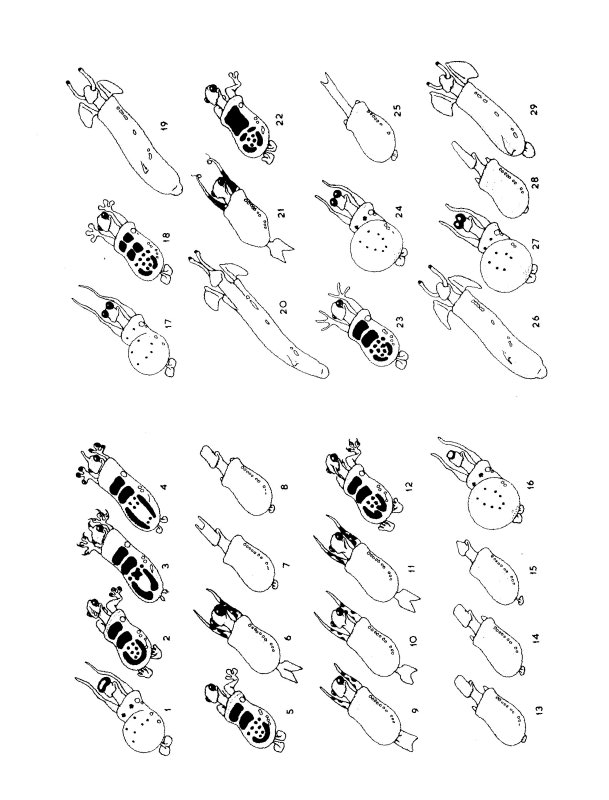
\includegraphics[scale=0.75]{./practica01/cami0.jpg}
% \resizebox{7in}{7in}{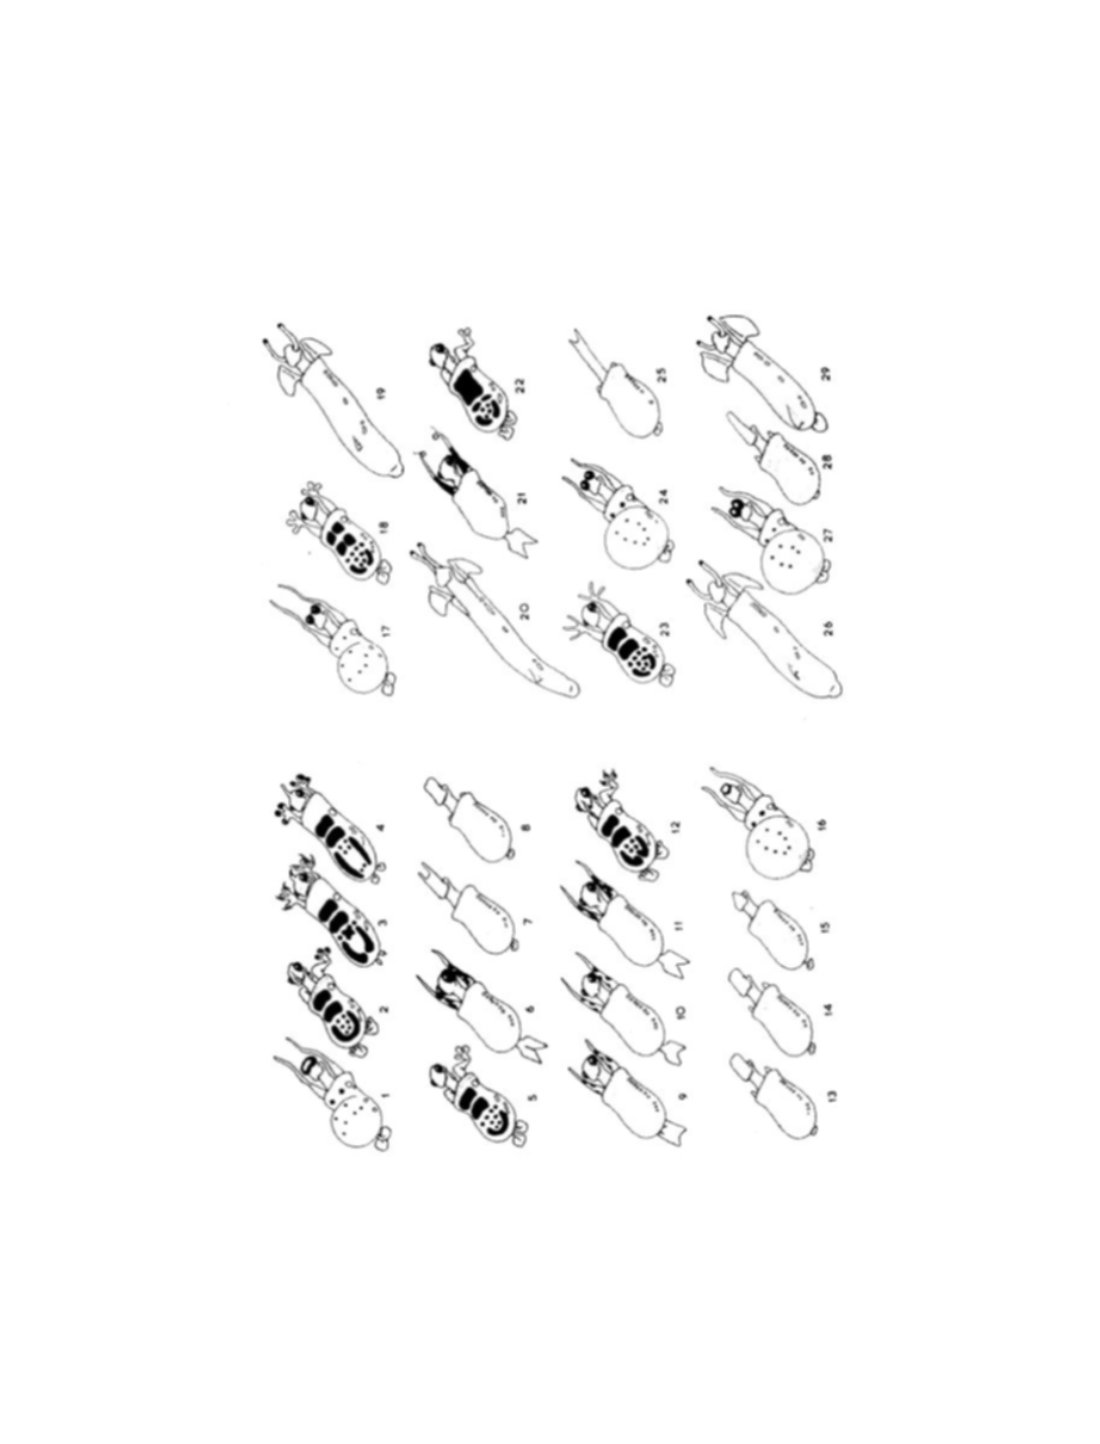
\includegraphics[]{camin.jpg}}
% \scalebox{0.80}[0.40]{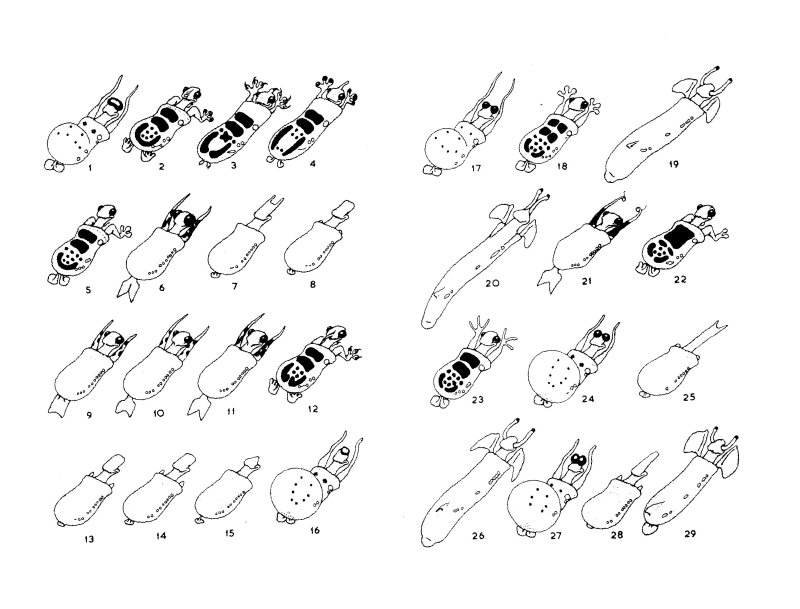
\includegraphics[clip,scale=1]{cami.jpg}}
% \resizebox{5in}{9in}{
\includegraphics[clip,scale=1]{2_p.jpg}}
% \includegraphics[bb= 600 920 100 0, scale=0.30]{portada.jpg}
% 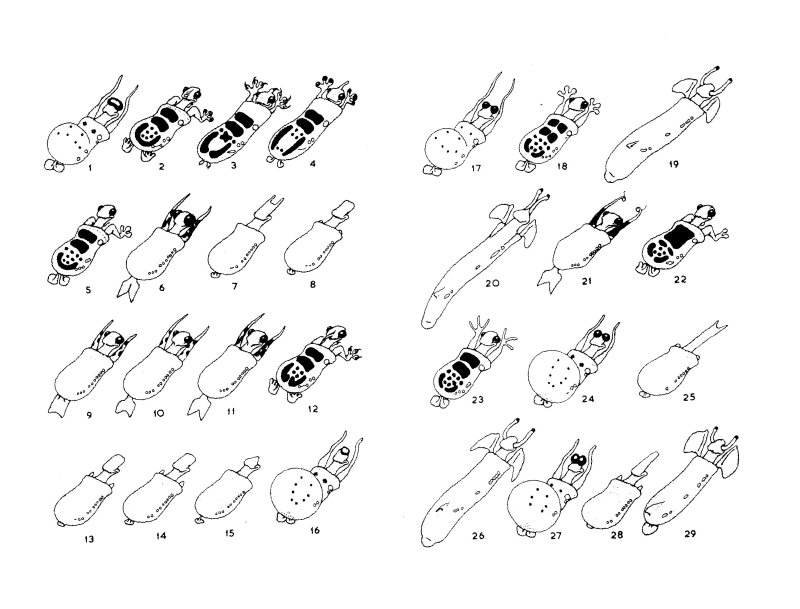
\includegraphics[bb= 100 200 100 0,scale=1]{cami.jpg}
% ,scale=0.5
\caption{Los Camin\'aculos, tomado de Sokal (1983) \\Copyright \textit{Society of Systematic Biologists}, se reproduce con permiso.}
% \vspace{-2mm}
\end{figure}



% 
\chapter{Matrices de datos}

\section*{Introducci\'on} 
\index{Caracter!Codificaci\'on} 

Una de las diferencias m\'as importantes entre los trabajos taxon\'omicos con un enfoque \textbf{cl\'asico} y los an\'alisis filogen\'eticos es que estos \'ultimos incluyen expl\'icitamente una matriz de datos donde se puede evidenciar los caracteres examinados, y c\'omo fueron interpretados.\\

B\'asicamente, la matriz de datos es una lista tabulada de las observaciones de los caracteres en los distintos taxa. Para facilitar su lectura y su uso en programas de an\'alisis filogen\'etico, los caracteres y sus estados son codificados como n\'umeros o como letras. Una vez construida, la matriz es el punto de partida para la b\'usqueda de \'arboles y la manera m\'as sencilla con la que otros investigadores pueden recuperar la informaci\'on recopilada durante el \textbf{an\'alisis de caracteres}\footnote{si desea puede ver nuestra visi\'on ampliada en Miranda et al., 2004.}.\\

Tal y como se hizo en la pr\'actica sobre selecci\'on de caracteres, lo que se busca es que el investigador sea consistente en la codificaci\'on de los caracteres, lo cual es importante en el manejo de caracteres inaplicables y no observados. Algunos autores los codifican de diferentes formas en la matriz (usualmente, con \textbf {-} y \textbf {?}) para facilitar la recuperaci\'on de informaci\'on (puede encontrar una discusi\'on m\'as completa en Strong \& Lipscomb, 1999),  otros autores, y en general los programas, no reconocen diferencia entre unos y otros, mientras que programas como \Pname{TNT} o \Pname{Poy} pueden reconocer como un quinto caracter los eventos de inserci\'on -perdida o gaps (Giribet \& Wheeler, 1999).\\
% Molecular Phylogenetics and Evolution
%Vol. 13, No. 1, October, pp. 132–143, 1999
%Article ID mpev.1999.0643, available online
%

Cuando se usan caracteres con m\'ultiples estados, es necesario clarificar cu\'ales fueron usados como aditivos y cu\'ales como no aditivos, o en el caso de haber sido recodificados, como se hizo esa codificaci\'on. Si se han codificado como aditivos, se debe indicar el ?`por qu\'e? de tal codificaci\'on e incluir los argumentos que muestren que los estados de car\'acter se hallan anidados entre s\'i, la aditividad puede generar al estrucutra en la topolog\'ia fianl, sin que haya relamente transformaciones qeu soporten los nodos.\\



\section*{T\'ecnicas}

Existen diferentes programas para manipular matrices de datos y \'arboles. Algunos de ellos permiten la interacci\'on matriz-\'arbol (
\Pname{WinClada}\footnote{\url{www.cladistics.com}}, 
\Pname{Mesquite}\footnote{\url{www.mesquite.org}}, 
\Pname{MacClade}\footnote{el programa no corre en versiones de MacOS X superiores a 10.6 (desde Lion en adelante)}, 
\Pname{R}\footnote{\Pname{R} es uno de los programas para an\'alis estad\'istico m\'as versatiles del momento, adem\'as de ser gratuito permite la implementaci\'on de m\'ultiples procesos de \'alculo, de tal manera que es posible realizar distintos tipos de operaciones y c\'alculos desde estadistica b\'asica hasta an\'alisis en evoluci\'on; sirve de plataforma para \Pname{ape} %faltan citas:
(Paradis et al., 2008), un m\'odulo que permite distintas acciones con matrices y \'arboles 
\url{cran.r-project.org}}  o 
\Pname{Seaview}\footnote{\url{doua.prabi.fr/software/seaview}}). En su mayor\'ia estos programas sirven de plataforma para manejar programas que realizan el an\'alisis filogen\'etico como tal. Muchos de los programas que manejan matrices est\'an dise\~nados b\'asicamente para alg\'un tipo particular de datos (por ejemplo, ADN) y aquellos que tienen un marco amplio se quedan cortos para manejar cierta clase de informaci\'on (por ejemplo, no interpretan la codificaci\'on IUPAC para polimorfismos de ADN).

Los programas pueden leer uno o varios formatos de archivos, pero solo algunos programas como \Pname{Mesquite} leen y escriben todos los formatos de datos; es importante revisar la compatibilidad de los programas para el manejo de archivos. En la mayor\'ia de ellos es posible exportar entre los diferentes tipos de datos, o por lo menos entre los m\'as usados. En general, la mayor parte de los programas trabaja bien con el formato NEXUS (Maddison, et al., 1997), 
%Maddison DR, Swofford DL, Maddison WP (1997). 
%"NEXUS: An extensible file format for systematic information". 
%Systematic Biology 46 (4): 590–621. doi:10.1093/sysbio/46.4.590. PMID 11975335.
tanto para exportar como para importar, aunque el formato es en ocasiones muy diferente y algunos programas pueden no identificarlo correctamente. El otro formato importante es el de Hennig86 o NONA, pero en muchos programas, especialmente moleculares, su uso no est\'a implementado.

Revise siempre la documentaci\'on del programa que desea usar y as\'i podr\'a estar seguro si el programa que va a utilizar cumple con los requisitos que usted necesita y cual es el formato de las matrices.

Existen listas de programas para an\'alisis filogen\'etico que pueden ser consultadas en internet, por ejemplo:


\url{http://evolution.genetics.washington.edu/phylip/software.html}
 
o en 

\url{http://taxonomy.zoology.gla.ac.uk/software/}

\section*{T\'ecnicas}

Abra el archivo de datos morfol\'ogicos para vertebrados \Datos{datos.vertebrados.xls} con un programa para hojas de c\'alculo y manuipule las matrices con \Pname{WinClada}, \Pname{Mesquite} o \Pname{TNT} para Windows:

\begin{enumerate}
	\item Anote cu\'ales caracteres son multiestado y cu\'ales son binarios.

	\item Identifique si hay o no caracteres aditivos.

	\item A partir de los datos, construya una matriz nueva (en \Pname{TNT} para Windows use el menu \Gui{Data - edit data}). 

	\item Dado que los programas no cuentan con opciones de salvado autom\'atico, peri\'odicamente salve la matriz.

	\item Nomine los terminales y los caracteres y sus estados. Explore diferentes formas de llevar esa tarea a cabo. 

	\item Suponga que algunos autores consideran que las plumas son escamas modificadas. Aceptando esa informaci\'on, recodifique la matriz y determine si el car\'acter es aditivo o no.

	\item Seleccione el \'ultimo car\'acter y col\'oquelo al principio de la matriz. 

	\item Introduzca un car\'acter nuevo en la posici\'on 4.

	\item Exporte la matriz en otros formatos, \Fname{NEXUS} si est\'a usando \Pname{WinClada}, \Fname{Nona} si est\'a usando \Pname{Mesquite}.

	\item Verifique la compatibilidad de los datos, abriendo la matriz en el programa correspondiente.

	\item Revise con un editor de texto los archivos que usted cre\'o, trate de identificar cu\'ales son las partes claves del formato\footnote{Aunque en general no se usan los editores de texto, este paso es cr\'itico para despu\'es ser capaz de rastrear los problemas que pueden tener las matrices de datos.}.

	\item Abra una de las matrices moleculares en cada programa y con un editor de texto y trate de identificar en qu\'e se diferencia de la matriz morfol\'ogica.

	\item en R:
	\begin{itemize}
		\item Instale en su ordenador la versi\'on m\'as reciente de R ($\ge$ 3.00-11). 

		\item Carge las bibliotecas \Rlib{ape} y \Rlib{phangorn}\footnote{La biblioteca \Rlib{phangorn} est\'a diseñada para an\'alisis filogen\'eticos que tiene como objetivo estimar \'arboles y redes,  utilizando diferentes m\'etodos como m\'axima verosimilitud,  parsimonia, distancia y conjugaci\'on de Handamard. Requiere las bibliotecas $"$ape$"$ y $"$rgl$"$,  y puede ser descargado desde \url {http://cran.r-project.org/web/packages/phangorn/index.html}}: 
		\Cmd{library(ape)}
		\Cmd{library(phangorn)}

		\item En caso de no tenerlas disponibles primero bajelas con la instrucci\'on:
		\Cmd{install.packages(c($"$ape$"$,$"$phangorn$"$), dependencies=T)}\footnote{La funci\'on \Rfunc{install.packages($"$Nombre\_paquete$"$)} permite hacer la descarga de los paquetes directamente del repositorio desde el entorno de R. Tambi\'en es posible hacer la descarga directamente de la pagina web e instalarlo desde cualquier directorio en el ordenador dando directamente la ruta a dicho sitio: 
		\Cmd{install.packages ($"$../usuario/R/Packages/Paquete.tar.gz$"$)}
		
		Tenga en cuenta que de este modo deberá descargar e instalar todas las dependencias requeridas por el paquete de manera independiente. El comando library() le permitir\'a cargar el paquete en el entorno de R para poder empezar a trabajar con todas sus utilidades.}

		\item Abra la matriz de datos en formato de texto simple y asignela a un objeto de R: 
		\Cmd{ datos $<-$ read.table($"$matriz.txt$"$)}

		\item Revise los nombres de las variables en la matriz con
		\Cmd{names(datos)}

		\item Revise los nombres de las terminales en la matriz con
		\Cmd{row.names(datos)}

		\item Abra la matriz de datos en formato \Fname{phylip} y asignela a un objeto de R: 
		\Cmd{datos.Phylip $<-$ read.phyDat($"$DNA1.phy$"$, format=$"$phylip$"$, type=$"$DNA$"$)} 

		\item Escriba en formato  \Fname{Nexus} la matriz leida anteriomente:
		\Cmd{write.nexus.data(datos.Phylip,file=$"$NuevaDNA1.nex$"$)}

		\item Abra la matriz escrita con \Pname{Winclada} o \Pname{Mesquite} y revise la conversi\'on.
	\end{itemize}

	\item En el directorio de datos existen dos matrices con distintos problemas \Datos{problema1.txt} y \Datos{problema2.txt}, intente abrir las matrices, busque  y corrija el error.\footnote{tradicionalmente, las terminaciones de los archivos son .ss en \Pname{WinClada}, .nex con \Pname{Mesquite} o \Pname{MacClade}, pero \textbf{debe} recordar que la terminaci\'on del archivo no es necesariamente el formato.}

\end{enumerate} 


Dependiendo de la plataforma que trabaje, usted tiene disponible distintos programas. \Pname{Mesquite} y  \Pname{R} son programas gratuitos y v\'alidos para todas las plataformas pero en general las b\'usquedas no son eficientes, aunque le permiten trabajar con varios tipos de datos e inreractuar directa o indirectamente con programas como \Pname{PAUP},\Pname{TNT} o \Pname{PhyML}. Sobre Windows usted cuenta con \Pname{WinClada} que funciona tanto en modo de manejo de edici\'on de matrices (\Gui {windada}) como en modo de edici\'on y manipulaci\'on de \'arboles; adem\'as, le permite hacer b\'usquedas con NONA, tambi\'en puede usar la versi\'on de Windows de \Pname{TNT} que tiene interface gr\'afica. Si usa Mac una opci\'on es \Pname{McClade}, el cual funciona como \Pname{Mesquite} pero es m\'as veloz y eficiente, aunque es muy factible que no lo pueda usar con la versi\'on actual de Mac OS X.


Revise la secci\'on de Programas de c\'omputo para ver los comandos que utilizar\'ia con un programa distinto a \Pname{Winclada/NONA}. En todos los casos familiar\'icese con los men\'us e instrucciones para abrir/cerrar y editar tanto matrices como \'arboles, tenga en cuenta que los manuales de los programas traen informaci\'on adicional, por lo tanto su lectura es una muy buena opci\'on.

\preguntaGral{
\begin{enumerate}

	\item Si desea transformar de un formato de matriz a otro usando exclusivamente editor de texto, ?`cu\'ales son los pasos a seguir? Ensaye la lista contruida con un ejemplo.

	\item Haga el listado de los aspectos comunes a todos los formatos de matrices.

	\item En el laboratorio anterior se insisti\'o en la claridad de los caracteres y sus estados. A la luz de los resultados obtenidos usando \'arboles y la matriz:

\begin{enumerate}

	\item ?`puede usted conectar la importancia del an\'alisis de caracteres con la forma como se interpretan los cladogramas?

	\item Revise su bibliograf\'ia, y de ser posible compare trabajos con y sin matriz expl\'icita. ?`Puede notar alguna diferencia?

	\item ?`Cree que es una ventaja incluir y publicar la matriz, o por el contrario es una desventaja?\\ 
\end{enumerate}


\end{enumerate}
}





\section*{Literatura recomendada}  

Maddison et al., 1997 [Una introducci\'on al formato NEXUS]. 

cita mesquite y sus bibliotecas

cita a NN? hennig? por que las matrices son importantes?

%
\chapter{\'Arboles}
\section*{Introducci\'on}

Una vez finalizado un an\'alisis filogen\'etico, el resultado es un agrupamiento que tradicionalmente se dibuja como un \'arbol donde los taxa usados estan como \emph{hojas} o \emph{terminales} del \'arbol. Las diferentes ramas se unen en \emph{nodos} o \emph{componentes}. As\'i, el agrupamiento ((Terminal 1, Terminal 2), Terminal 3) puede representarse con el \'arbol:

\begin{center}
%
% http://tex.stackexchange.com/questions/2340/how-to-make-a-3-level-deep-tree-with-tikz
%
\begin{tikzpicture}[level distance=3cm,
  level 1/.style={sibling distance=9cm},
  level 2/.style={sibling distance=6cm}]
  \node {Ra\'iz}
    child {node {Terminal 3}}
    child {node {Nodo interno 1}
    	child {node {Terminal 1 = nodo (hoja)}}
      	child {node {Terminal 2}}
    };
\end{tikzpicture}
\end{center}

Es importante diferenciar entre el \textbf{contenido} del nodo, que son los terminales que forman el nodo (el nodo interno 1 tiene dos terminales: 1 y 2), y la \textbf{informaci\'on} del nodo, que es c\'omo est\'an organizados estos terminales en terminos de grupos o clados anidados (Nelson, 1979). En general, para muchos autores un componente representa un grupo monofil\'etico (i.e., definici\'on \emph{topol\'ogica} de monofilia).

En clad\'istica, los \'arboles son tambi\'en conocidos como \textbf{cladogramas} y el t\'ermino es usado sin distinci\'on. En clad\'istica (pero no en otras metodolog\'ias) los cladogramas deben tener transformaciones de caracteres en nodos (nodos soportados), en caso de no tener transformaciones, el nodo no est\'a soportado o es un nodo de longitud cero, es decir, es un artefacto de los programas usados para obtener los \'arboles (v\'ease Coddington \& Scharff, 1994; Goloboff, 1998). El n\'umero de transformaciones es un estad\'istico importante que hay que tener en cuenta y se usa como criterio para seleccionar entre diferentes cladogramas, se escoge la topolog\'ia que sugiere el  menor n\'umero de transformaciones. En los m\'etodos estad\'isticos generalmente es importante la longitud de las ramas, esta suele representarse como una probabilidad o frecuencia de transformaciones y suelen presentarse los \'arboles con una escala que muestra la longitud de ramas; s\'olo la dimensi\'on que va de las ramas a los terminales tiene importancia en ese caso, el $"$ancho$"$ del \'arbol se usa para acomodar los diferentes terminales usados. En los cladogramas, las dimensiones no tienen ning\'un significado especial.


\section*{T\'ecnicas}

Una forma de expresar los \'arboles en formato de texto (por ejemplo para usar con programas o para el resumen de un art\'iculo) es la notaci\'on de par\'entesis, donde los par\'entesis limitan los nodos; dependiendo de los autores o los programas, los grupos hermanos son separados por espacios, comas o s\'imbolos de suma, por ejemplo (a (b c)), es equivalente a (a+(b+c)) y a (a, (b, c)), tenga en cuenta que en los \'arboles filogen\'eticos el orden de los terminales, sin cambiar la topolog\'ia, no altera el contenido del \'arbol, por ejemplo (a (b c)) es exactamente igual a ((c b) a) y a ((b c) a).

Existen diferentes programas para manipular y generar \'arboles; la mayor\'ia de ellos permiten interacci\'on matriz-\'arbol, mientras que otros solo utilizan \'arboles. En general, los programas de an\'alisis filogen\'etico permiten manipular \'arboles en un esquema gr\'afico rudimentario. Algunos programas permiten guardar informaci\'on adicional a la topolog\'ia en el mismo \'arbol como la longitud de la rama que conduce al nodo o terminal o una etiqueta. Los programas que pueden trabajar independientemente de la matriz suelen estar dise\~nados para la impresi\'on o exportaci\'on gr\'afica de los \'arboles, soportando cambios de topolog\'ia, longitudes y etiquetas de las ramas, pero no transformaciones de caracteres.

Dependiendo de la plataforma que trabaje, usted tiene disponible distintos programas: \Pname{Mesquite}, \Pname{R}\footnote{\url{cran.r-project.org}} y \Pname{Figtree}\footnote{\urlt{tree.bio.ed.ac.uk/software/figtree/}} son v\'alidos para todas las plataformas (adicionalmente son gratuitos). \Pname{Mesquite} es muy lento si su m\'aquina es lenta (requiere de la m\'aquina virtual de Java). Sobre Windows usted cuenta con \Pname{WinClada} (requiere la matriz de datos), su interfaz de impresi\'on requiere mucha pr\'actica (no es intuitiva). Otras alternativa, si usa Linux, pueden ser \Pname{NJPlot o GNUplot}. Para la impresi\'on final del \'arbol para publicaci\'on, una opci\'on puede ser \Pname{R}, que aunque es poco intuitivo al iniciar, logra resultados fianles de mejor calidad que otros programas.

En general, la manipulaci\'on de arboles se activa con un men'u (en \Pname{WinClada} \Gui{Edit/Mouse}, en \Pname{FigTree} directamente como barra de herramientas en la ventana; en \Pname{Mesquite} se usa el men\'u de herramientas de la ventana de edici'on de \Pname{TreeView}). Las acciones se realizan al seleccionar con el rat\'on la rama (\Pname{WinClada}) o arrastrando las ramas (para moverlas en \Pname{Figtree}). M'as que comandos, en esta pr\'actica es importante manipular el rat\'on.}}


\begin{enumerate}

	\item Desde \Pname{WinClada+NONA}, \Pname{Mesquite} o \Pname{TNT}
	\begin{enumerate}
		\item Revise los archivos de datos con editor de texto y con le programa seleccionado abra una matriz de datos que contenga tanto datos como \'arboles.
		\item Establezca la forma de obtener informaci\'on sobre los \'arboles, en un principio los costos o longitud del \'arbol.
		\item Cambie de posici\'on algunos nodos o terminales de la topolog\'ia, y observe c\'omo cambia la longitud del cladograma y los estados asignados a los nodos o la forma como los caracteres son mapeados, pruebe tambi\'en moviendo ramas completas.
	\end{enumerate}

	\item En \Pname{Mesquite} y \Pname{TNT} (para Windows) usted puede mover ramas completas; en \Pname{TNT} (para Windows) use el menu \Gui {Trees - view} y seleccione con el bot\'on izquierdo del rat\\'on el clado a mover (el clado queda marcado en rojo), se\~nale con el rat\'on el destino usando el bot\'on derecho.
	\item Desde \Pname{WinClada} o \Pname {TNT} (para Windows), haga una b\'usqueda de cladogramas para la matriz de vertebrados que contruy\'o en la pr\'actica de matrcies, use los par'ametros por omisi\'on (men\'u \Gui{Analize} / \Gui{heuristics}, \Gui{traditional search}).
	\item En \Pname{Mesquite} o \Pname{Figtree}:
	\begin{enumerate}
		\item Cambie el orden de los terminales sin cambiar la topolog\'ia (las relaciones entre terminales) del \'arbol.
		\item Coloque etiquetas en los nodos, y salve el \'arbol.
		\item Revise ese archivo en un editor de texto para determinar c\'omo se colocaron tanto las etiquetas como las longitudes.
		\item Abra el \'arbol con longitud de ramas.
	\end{enumerate}


	\item En \Pname{Mesquite} o \Pname{WinClada} abra el archivo \Datos{datos.conarbol.dat}:
	\begin{enumerate}
		\item Indique la cantidad de \'arboles presentes y la longitud de los mismos.
		\item Examine las agrupaciones obtenidas e identifique los caracteres que soportan los nodos.
		\item Mapee los caracteres en los \'arboles usando distintos tipos de optimizaciones: en \Pname{WinClada} ACCTRAN (=fast), DELTRAN (=slow) y no ambigua, En \Pname{TNT} (para Windows) (\Gui{Optimize $>$ Character $>$ Reconstructions} y seleccione un solo \'arbol y algunos caracteres) y en \Pname{Mesquite}: Dollo e Irreversible (C-S); revise c\'omo cambian las optimizaciones en los distintos nodos.
		\item Revise de nuevo el efecto en la longitud de los \'arboles de las siguentes modificaciones:
		\begin{enumerate}
			\item Cambie la ra\'iz del \'arbol.
			\item Cambie de posici\'on nodos y terminales.
			\item Seleccione un nodo y colapselo.
		\end{enumerate}
	\end{enumerate}

	

	\item \En \Pname{R}:
	\begin{enumerate}

		\item Lea el archivo con \'arboles \Datos{arbol.r.tre} use las instrucciones:
		\Cmd{library(ape); arbol <- read.tree($"$arbol.r.tre$"$)}
		\item Grafique el objeto \Rdatos{arbol} use las instrucciones, que por defecto dibuja el \'arbol con longitud de ramas o como un filograma:
		\Cmdi{  
			\begin{itemize}[label=$>$]
  				\item plot(arbol) o 
  				\item plot.phylo(arbol)
  			\end{itemize}}

		\item Para graficar el \'arbol sin incluir la longitud de ramas  use las instrucciones:
		\Cmd{plot(arbol,use.edge.length=FALSE)} 
		\item Para asignar las longitudes de las ramas como r\'otulos de los nodos y graficarlos use las instrucciones:
		\Cmdi{  
			\begin{itemize}[label=$>$]
  				\item arbol\$node.label<-arbol\$edge.length
  				\item plot(arbol,show.node.label=TRUE)
  			\end{itemize}
  			}
		\item Para graficar el \'arbol con t\'itulo de gr\'afica, colores de ramas y tipo cladograma use las instrucciones:
		\Cmd{plot(arbol, type="cladogram",main="\'Arbol 1",
		edge.col=c("red","blue","cyan"))}
		\item Para obtener la longitud del \'arbol, lea la matriz de datos \Datos{matriz.r.phy} a un objeto que se llame \Rfunc{MatrizDatos} y use la funci\'on \Rfunc{parsimony()}:
		\Cmd{parsimony(arbol,MatrizDatos)}
	\end{enumerate}	


\pregunta{\begin{enumerate}
	\item Al hacer una b\'usqueda por defecto ?`Usted y sus compan\~neros obtienen las mismas topolog\'ias y los mismos caracteres que soportan los grupos?.
	\item Al cambiar la aditividad/no aditividad de un caracter  ?`Cambia esto la forma como se mapean? Haga este ejercicio para varios caracteres, tanto binarios como multiestado.
	\item Si cambia la ra\'iz, ?`cambia la longitud? ?`Por qu\'e cree que se presenta el resultado que obtuvo? ?`Es (y por qu\'e) una ventaja o una desventaja?
	\item Examine sus caracteres y cambie su aditividad-no aditividad. ¿Cambia esto la forma como mapean? Haga este ejercicio para varios caracteres, binarios y multiestado.
	\item Si cambia la ra\'iz, ¿cambia la longitud? ¿Por qu\'e cree que se presenta el resultado que obtuvo? ¿Es (y por qu\'e) una ventaja o una desventaja?
	\item Dibuje el siguiente cladograma:\\ 
	\begin{small}
	\emph{(Lampreas (Tiburones (Esturi\'on Tele\'osteos) (Celacanto (Peces-pulmonados (Anfibios (Mam\'iferos (Tortugas (Lagartos (Cocodrilos Aves)))))))))}
	\end{small}
	\item Si la ra\'iz esta colocada entre Aves y Cocodrilos, ¿c\'omo es la topolog\'ia resultante?
	\item Convierta la topolog\'ia dibujada a notaci\'on de par\'entesis.
\end{enumerate}}


\end{enumerate}


\preguntaGral{Aparte de no tener un an\'alisis expl\'icito, existe una gran diferencia entre los \'arboles filogen\'eticos actuales y sus $"$equivalentes$"$ usados por algunos tax\'onomos (por ejemplo, Haeckel, Romer, etc.) ?`Es usted capaz de descubrirla? \textbf{Clave}: intente dibujar alguno de esos \'arboles al estilo actual.}

\section*{Literatura recomendada}

Page \& Holmes, 1998 [El cap\'itulo 2 esta dedicado a los \'arboles y presenta muy buenas ilustraciones, Tambi\'en puede consultar la p\'agina de docencia de Rod Page (\url{taxonomy.zoology.gla.ac.uk/teaching/index.html})].

%% todo: revisar validez de pagina rod page docencia


%

\chapter{B\'uquedas mediante parsimonia} % (fold)
\label{cha:parsimonia}

\section*{Introducci\'on} 

Un discusi\'on constante en sistem\'atica es como seleccionar cladogramas, por ejemplo, {\color{red}Hennig (1968)} plantea relaciones mediante la agrupaci\'on por sinapomorfias, no es muy expl\'icito a lo que refiere la obtenci\'on del cladograma. {\color{red}Camin \& Sokal (1965)} posiblemente fueron los primeros en sugerir el uso de la \textit{parsimonia} como un posible m\'etodo para hacer esta selecci\'on; desde entonces el cladograma seleccionado es aquel que minimiza la cantidad de transformaciones, es decir \textit{el cladograma m\'as parsimonioso}. Posteriormente, esta t\'ecnica fue generalizada usando diferentes tipos de optimizaci\'on: unas de las mas conocidas e implementadas son: \textit{la optimizaci\'on de Wagner y la optimizaci\'on de Fitch} {\color{red}(Wagner, 1961; Kluge \& Farris, 1969; Farris, 1970; Farris et al., 1970; Fitch, 1971)}.


La b\'usqueda del cladograma mas parsimonioso es m\'as compleja a mediada que se agregan terminales,  por ello los algoritmos para b\'usquedas exactas solo son viables con pocos terminales (aprox. 20-30),  despu\'es de este n\'umero el espacio de \'arboles es tan grande que es imposible una b\'usqueda exacta (dado que es un problema NP-Completo). Por esta raz\'on se utilizan b\'usquedas heur\'isticas que permiten obtener respuestas generalmente cercanas al \'optimo global,  y pese a que estas soluciones no proporcionan con certeza la soluci\'on \'optima, se obtienen resultados  dif\'iciles de superar.
%{\color{red} Cita}

La forma m\'as sencilla de elaborar cladogramas es usando el algoritmo de Wagner: como el orden de entrada de los taxa afecta la topolog\'ia,  se realiza una aleatorizaci\'on de tal secuencia de entrada {\color{red} (Dayo, 1969)},  la cual puede estar seguida de permutaciones de ramas. Sin embargo,  este ultimo paso para matrices muy grandes consume gran cantidad de tiempo; esto se debe repetir m\'ultiples veces para evitar caer en "\'optimos locales". Con este m\'etodo es posible una soluci\'on optima incluso para matrices de 80 a 100 terminales. Problemas mas grandes requieren nuevas estrategias,  algunas de ellas derivadas de la cristalizaci\'on simulada,  aceptando moment\'aneamente cladogramas sub\'optimos para iniciar desde ellos la permutaci\'on de ramas. Otros utilizan combinaciones bien sea entre b\'usquedas exhaustivas o entre b\'usquedas sobre reducciones de la matriz.

Una nueva ventana para las matrices cada vez m\'as grandes (por ejemplo matrices moleculares con m\'as de 1000 terminales),  es tratar de identificar el acuerdo entre distintas r\'eplicas de b\'usquedas parciales,  en vez de buscar la soluci\'on \'optima {\color{red}(e.g. Farris et al.,  1996; Farris,  1997; Goloboff,  1997b; Goloboff \& Farris,  2001)}. 

En terminos de programas de computo,  la mejor opci\'on para programas gratuitos es \Pname{TNT}; este es el programa m\'as  completo para an\'alisis clad\'istico,  usted lo encuentra disponible para Windows/DOS,  MacOSX y Linux,   es bastante r\'apido,   adem\'as de tener implementado ratchet y las nuevas b\'usquedas.  \Pname{NONA} otra posible opci\'on puede manejarse como buscador con WinClada (para Windows),  es buena idea que se familiarice con estos programas y la l\'inea de comandos, las b\'usquedas son m\'as eficientes desde la l\'inea de comandos. \Pname{PAUP*}  tambien est\'a disponible como ejecutable en varias plataformas (Windows,  Mac\footnote{debe revisar la compatibilidad con las \'ultimas versiones de Mac OS X, ya que el programa no se ha actulizado en los \'ultimos a\~nos} y Linux).  \Pname{PAUP*}  no solo usa parsimonia sino distancias y m\'axima verosimilitud, aunque para parsimonia es menos vers\'atil que \Pname{TNT}.  \Pname{TNT} est\'a dice\~nado para b\'usquedas exhaustivas en matrices grandes, la velocidad y sistema de macros son sorprendentes; pero,  por lo menos hasta el momento, no hace b\'usquedas mediante ML.


\section*{T\'ecnicas}

El algoritmo de Wagner es la base para las b\'usquedas actuales. Para evitar el problema del orden de entrada de los datos,   los taxa se  seleccionan al azar (RAS\footnote{En algunos escenarios se peude comenzar con un \'arbol al azar que ser\'a mejor punto de inicio que un \'arbol de Wagner, ver Goloboff (2014).}),
    %Hide and vanish: data sets where the most parsimonious tree is known but hard to find, and their implications for tree search methods
    %Molecular Phylogenetics and Evolution
la mayor parte de los programas actuales tienen esta opci\'on: inician con una \textbf{semilla} determinada para el generado de n\'umero aleatorio y aseguran que la b\'usqueda sea exactamente igual a otra que tenga el mismo de inicio (semilla del generador de n\'umeros seudo-aleatorios). Una vez construido un cladograma,  este suele ser sometido a permutaci\'on de ramas para mejorar su calidad. B\'asicamente se toma un nodo (sub\'arbol) y es eliminado del cladograma principal,   luego se prueba si al unirlo en diferentes lugares del cladograma principal disminuye la longitud con respecto al cladograma original. Se puede permutar ramas de varias formas;  las m\'as comunes son unir el nodo a las diversas ramas del cladograma principal (subpoda y replantado,  SPR por sus siglas en Ingl\'es)\index{B\'usqueda!SPR},  o intentar otros puntos de uni\'on dentro del sub\'arbol y cambiar la topolog\'ia (bisecci\'on y reconexi\'on de \'arboles,  TBR). En general,   la mayor parte de los programas utilizan TBR, \index{B\'usqueda!TBR} puesto que el tiempo de permutaci\'on entre ambas t\'ecnicas es casi igual y TBR es mucho m\'as eficiente.


\begin{itemize}
  \item Con \Pname{NONA/Winclada,  TNT,  POY} y \Pname{PAUP*}

	Construya una tabla (Ap\'endice 1) donde pueda registrar la informaci\'on de tiempos de b\'usqueda,   n\'umero de cladogramas y costo del mejor cladograma,  para cada una de las siguientes b\'usquedas:
 

	\begin{enumerate}
	  \item  {B\'usquedas por omisi\'on}

  		Ejecute el archivo datos.chica.dat siguiendo los comandos:

  		\begin{itemize}
  			\item  \Pname{NONA/Winclada}

  				\Gui{File/File open}
  			
  				\Gui{Heuristic Search}

  			\item  \Pname{TNT}
  				\Cmd{proc nombre\_archivo;}
  				\Cmd{mult;}

  			\item  \Pname{POY}
  				\Cmd{read( $'$nombre\_archivo')} 
  				\Cmd{build()}
  				\Cmd{swap()}


  			\item  \Pname{PAUP*}
  				\Cmd{set criterion=parsimony}
  				\Cmd{exec nombre\_archivo}
  				\Cmd{hsearch}

  		\end{itemize}

        \pregunta{%{Preguntas}\\
          \begin{itemize}
    		    \item ?`Qu\'e tipo de informaci\'on puede obtener cuando carga el archivo de datos?
    		    \item ?`C\'ual es la b\'usqueda por omisi\'on en cada programa utilizado?
    	   \end{itemize}
        }


	  \item{B\'usquedas modificadas}

		Con el archivo el datos \RDatos{datos.chica.dat} realice las siguientes b\'usquedas,  modificando los comandos que sean necesarios.
 

 \begin{table}[H]
 \centering
 \begin{tabular}{|c|c|}
 \hline
  N\'umero de r\'eplicas & \'arboles retenidos/r\'eplica\\
 \hline
  5 & 1\\ 
   \hline
  5 & 100\\
   \hline 
  10& 1\\ 
   \hline
   10& 100\\
    \hline 
  100 & 1 \\
   \hline
   100 & 100 \\
  \hline
  
  
 \end{tabular}
 
 \end{table}
 
	El manual de cada programa especifica los comandos a modificar para hacer dichas b\'usquedas como por ejemplo: Para b\'usquedas con \Pname{NONA},  el comando m\'as usado es mult*  para las b\'usquedas iniciales,   max*  para permutar ramas (requiere \'arboles) y nix*  para ratchet. En \Pname{TNT} tambi\'en se puede usar mult; la permutaci\'on de ramas es con bbreak.  En \Pname{PAUP*} debe definir el criterio de  b\'usqueda: parsimonia usando set criterion=parsimony,  y la b\'usqueda con hsearch tanto para \'arboles de Wagner como para permutar ramas; en este \'ultimo caso use hsearch start=current.

	Para los archivos de macros de \Pname{TNT} use la instrucci\'on run seguida del nombre del archivo; en este caso pauprat.run y los par\'ametros run pauprat.run 10 5; TNT usa pesos de 1 y 2 en el archivo de salida,  pauprat.
 
 

	%{Preguntas}
  \pregunta{
    \begin{itemize}
		  \item 	Utilice un manejador gr\'afico que le permita visualizar la tendencia en los datos obtenidos.
		  \item  ?`Encontr\'o alguna tendencia en t\'erminos de tiempos o costos,  al aumentar el n\'umero de replicas?
	   \end{itemize}
  }



	\item{B\'usquedas con RACHET}

	Utilizando el mismo archivo.dat,  realice las siguientes b\'usquedas:

 \begin{table}[H]
 \centering
 \resizebox{13cm}{2cm}{
 
 \begin{tabular}{|c|c|c|}
 \hline
  N\'umero de B\'usquedas continuas & N\'umero de r\'eplicas/B\'usqueda&  N\'umero iteraciones en RACHET\\

 \hline
  1 & 5 & 50\\ 
 \hline
  1 & 5 & 100\\ 
 \hline
  1 & 10 & 50\\ 
 \hline 
  1 & 50 & 50\\  
 \hline
  5 & 1 & 5\\
 \hline
 20 & 1 & 5\\
 \hline

 \end{tabular}
 }
 \end{table}

	En problemas m\'as complejos de 100 o m\'as terminales, se requiere utilizar t\'ecnicas m\'as sofisticadas para obtener resultados satisfactorios. La m\'as sencilla es el rastrillo o pi\~n\'on (\textit{ratchet}\index{B\'usqueda!Ratchet} en ingl'es) {\color{red}(Nixon,  1999; Quickle,  2001)},  la cual es una forma simple de implementar una cristalizaci\'on simulada. El m\'etodo consiste en usar un \'arbol ya elaborado (por ejemplo con Wagner + TBR),  perturbar la matriz de datos (con eliminaci\'on o repesado de caracteres), permutar las ramas del \'arbol para obtener el \'optimo de la nueva matriz,  volver la matriz a su estado original y buscar el \'arbol \'optimo con permutado de ramas (todo ese proceso es una iteraci\'on,  la cual se repite \textbf{n} veces). El rastrillo es eficiente usando solo unos pocos \'arboles por iteraci\'on y permutando una cantidad intermedia de caracteres (entre 10-25\%), en general, mejora dr\'asticamente el ajuste de los cladogramas en las primeras iteraciones (Nixon,  1999).
 
	Para producir nuevas mejoras en el ajuste de cladogramas con n\'umeros mayores a 500 terminales,  los m\'etodos m\'as eficientes parecen ser la \''deriva de \'arboles\'',  que es una implementaci\'on m\'as expl\'icita de la cristalizaci\'on simulada (es decir aceptar soluciones ligeramente sub\'optimas con una determinada probabilidad,  y a medida que el an\'alisis avanza,  se disminuye la probabilidad de aceptaci\'on de los sub\'optimos),  y la fusi\'on de \'arboles,  que utiliza lo mejor de diferentes soluciones. Una revisi\'on completa de estos m\'etodos se puede consultar en {\color{red} Goloboff (1999)}.
  
  
%\subsubsection*

    %{Preguntas}
  \pregunta{
	 \begin{itemize}
		  \item ?`C\'ual es y que hace el comando que permite hacer b\'usquedas con la t\'ecnica RACHET en cada programa?
		  \item ?`Cada b\'usqueda o r\'eplica es independiente de otra?
		  \item ?`Hay alg\'un efecto en el resultado al hacer varias b\'usquedas continuas con el mismo n\'umero de r\'eplicas o es suficiente una sola b\'usqueda con m\'ultiples replicas? Realice b\'usquedas adicionales con par\'ametros diferentes que le permitan responder estas preguntas. Utilice un manejador grafico donde pueda visualizar la tendencia de los datos obtenidos.
	 \end{itemize}
   }


\end{enumerate}

  
\item An\'alisis Filogen\'etico en R, Bibliotecas y dependencias

\begin{enumerate}
  \item Instale en su ordenador la versi\'on m\'as reciente de R ($\ge$ 3.00-11). 
  \item Carge, y de ser necesario instale,  la biblioteca \Rlib{"phangorn"}
  \Cmd{install.packages ("phangorn", dependencies=TRUE)}
  \Cmd{library (phangorn)}
  \item{Lectura del alineamiento o matriz y formato de escritura}
  \begin{enumerate}
    \item   Cargue el alineamiento o la matriz llamada chars2.txt  y defina los argumentos requeridos para que esta pueda ser le\'ida. 
    \item Escr\'ibala como formato NEXUS utilizando el nombre primates.nex:
    \Cmd{primates <- read.phyDat ($"$chars2.txt$"$, format=$"$phylip$"$,  type=$"$DNA$"$)}
    \Cmd{write.nexus.data (primates, file="primates.nex")}
    \item Revise la matriz primates.nex con un editor de texto,  identifique las particularidades del formato en R y si este archivo es similar al generado por winclada.
  \end{enumerate}


La funci\'on \Rfunc{read.phyDat()} permite leer diferentes tipos de caracteres como $"$DNA$"$,  $"$AA$"$,  $"$CODON$"$ o $"$USER$"$,  este \'ultimo es definido por el usuario. Posteriormente, el vector denominado primates es escrito en otro formato diferente al formato phyDat; la funci\'on \Rfunc{write.nexus.data()} escribe un archivo formato NEXUS a partir de un vector de secuencias. Los argumentos de una funci\'on pueden ser consultados con el comando \Rfunc{args(Nombre\_funci\'on)} o con el comando de ayuda \Rfunc{?Nombre\_funci\'on}.


%\subsubsection*

{Preguntas}

?`Qu\'e otras funciones en otras bibliotecas permiten leer y/o escribir archivos tipo Nexus,  Fasta,  Phylip,  Clustal,  Sequential e Interleave?\\

\item{Topolog\'ias iniciales}

Estime la matriz de distancia,  realice el an\'alisis de agrupamiento y grafique para un posterior an\'alisis.

\Cmd{dm <- dist.dna (as.DNAbin(primates))} 
\Cmd{treeUPGMA <- upgma (dm)}
\Cmd{treeNJ <- NJ(dm) }
\Cmd{plot (treeUPGMA,  main=$"$UPGMA$"$,  cex = 0.8)}
\Cmd{plot (treeNJ,  $"$unrooted$"$,  main=$"$NJ$"$,  cex = 0.5) }


La funci\'on \Rfunc{dist.dna()} permite obtener una matriz de distancias por pares de secuencias de ADN,  bajo un modelo evolutivo determinado. 
Actualmente es posible estimar esta matriz bajo 11 modelos evolutivos diferentes,  adem\'as permite estimar la varianza entre distancia y el valor de gamma. Existen varios m\'etodo de agrupamiento por distancia para obtener la topolog\'ia inicial,  entre ellos los algoritmos UPGMA (=Unweighted Pair Group Method with Arithmetic Mean),  WPGMA (=Weighted Pair Group Method with Averaging),  NJ (Neighbor Joining) y UNJ (Unweighted Neighbor Joining); en este caso las funciones \Rfunc{upgma()} y \Rfunc{NJ()} permiten construir \'arboles de distancia bajo sus caracter\'isticas espec\'ificas,  los cuales pueden ser visualizados con la funci\'on \Rfunc{plot()}.


\Cmd{treeRAM <- random.addition(primates,  method=$"$fitch$"$) }
\Cmd{plot (treeRAM,  main=$"$UPGMA$"$,  cex = 0.8)}

La funci\'on  \Rfunc{random.addition()}, permite definir los \'arboles iniciales de los cuales parte el an\'alisis de parsimonia.

{Preguntas}

?`En que difiere cada \'arbol obtenido?

?`En que consiste el m\'etodo de FICHT y el m\'etodo de SANKOFF?

?`Que hacen los algoritmos de agrupamiento UPGMA,  WPGMA,  NJ y UNJ?

?`En que consiste el m\'etodo de construcci\'on de \'arboles de random.addition?


\item{Parsimonia y optimizaci\'on}
 
A partir de la matriz de dataos primtes.nex y las topolog\'ias construidas,  calcule la longitud  de los \'arboles y obtenga el \'arbol de menor costo o score.
\Cmd{parsimony (treeUPGMA,  primates)}
\Cmd{parsimony (treeNJ,  primates)}
\Cmd{parsimony(treeRAM, primates)}

La funci\'on \Rfunc{parsimony()} permite obtener el \'arbol de menor longitud utilizando el algoritmo del m\'etodo SANKOFF o de FITCH,  en este caso es una busqueda por omisi\'on dado que no se especifican los argumentos.
 

Optimice cada topolog\'ia obtenida en el punto C,  utilizando el m\'etodo de optimizaci\'on por omisi\'on,  optimizaci\'on por SPR y optimizaci\'on por NNI. Registre sus resultados en el Ap\'endice 2.

\item Optimizaci\'on por omisi\'on


\Cmd{optParsUPGMA <- optim.parsimony (treeUPGMA,  primates)}


\Cmd{optParsNJ <- optim.parsimony (treeNJ,  primates)}


\Cmd{optParsRAM <- optim.parsimony (treeRAM,  primates)}


\item Optimizaci\'on con rearreglo de ramas espec\'ifico


\Cmd{optParsUPGMA\_SPR <- optim.parsimony (treeUPGMA,  primates, rearrangements=$"$SPR$"$)}


\Cmd{optParsUPGMA\_NNI <- optim.parsimony (treeUPGMA,  primates, rearrangements=$"$NNI$"$)}

%\normalsize

La funci\'on optim.parsimony() intenta encontrar el o los \'arboles mas parsimoniosos utilizando los m\'etodos de rearreglos NNI y SPR.

%\subsubsection*

\pregunta{
?`En que difieren los m\'etodos de rearreglos NNI,  SPR y TBR?

?`Cuales  son los argumentos por omisi\'on de las funciones \Rfunc{parsimony()} y \Rfunc{optim.parsimony()}?
}

\item{Parsimonia usando Rachet} 



Utilice el m\'etodo Rachet en parsimonia para hacer las b\'usquedas del o los \'arboles de menor costo. Complete la tabla del Ap\'endice 3 creando nuevas l\'ineas de c\'odigo para hacer las b\'usquedas con los \'arboles obtenidos en el proceso anterior,  use los siguientes par\'ametros para las  b\'usquedas.

\item B\'usqueda con Rachet utilizando los \'arboles iniciales y optimizando con el m\'etodo de rearreglos NNI.


\Cmd{pratchet(primates,  start=treeUPGMA,  method="fitch",  maxit=100,  k=5,  trace=1,  all=FALSE, rearrangements="NNI")}

\item B\'usqueda con Rachet utilizando los \'arboles iniciales y optimizando con el m\'etodo de rearreglos SPR.


\Cmd{pratchet(primates,  start=treeUPGMA,  method="fitch",  maxit=100,  k=5,  trace=1,  all=FALSE, rearrangements="SPR")}

\item B\'usqueda con Rachet utilizando los \'arboles optimizados con NNI y optimizando con el m\'etodo de rearreglos NNI.


\Cmd{pratchet(primates,  start=optParsUPGMA\_NNI,  method="fitch",  maxit=100,  k=5,  trace=1,  all=FALSE, rearrangements="NNI")}


\item B\'usqueda con Rachet utilizando los \'arboles optimizados con NNI y optimizando con el m\'etodo de rearreglos SPR.


\Cmd{pratchet(primates,  start=optParsUPGMA\_NNI,  method="fitch",  maxit=100,  k=5,  trace=1,  all=FALSE,  rearrangements="SPR")}



\item B\'usqueda con Rachet utilizando los \'arboles optimizados con SPR y optimizando con el m\'etodo de rearreglos NNI


\Cmd{pratchet(primates,  start=optParsUPGMA\_SPR,  method="fitch",  maxit=100,  k=5,  trace=1,  all=FALSE, rearrangements="NNI")}


\item B\'usqueda con Rachet utilizando los \'arboles optimizados con SPR y optimizando con el m\'etodo de rearreglos SPR


\Cmd{pratchet(primates,  start=optParsUPGMA\_SPR,  method="fitch", maxit=100,  k=5,  trace=1,  all=FALSE, rearrangements="SPR")}



\Rfunc{pratchet()} hace b\'usquedas usando el m\'etodo de Rachet, estas b\'usquedas son hechas a partir de un \'arbol inicial ya sea optimizado o no,  aunque es preferible partir de un \'optimo ya dado. Tambi\'en puede iniciar haciendo una b\'usqueda para obtener el \'arbol o los \'arboles de partida, aplicar el m\'etodo de rachet y \'optimizar.


%\subsubsection*

\pregunta{
?`Hay diferencias entre las b\'usquedas con rachet en t\'erminos de costos o tiempo?
Escriba y ejecute la l\'inea de c\'odigo que le permitir\'ia realizar una b\'usqueda con: 70 iteraciones en Rachet, Metodo SANKOFF, rearreglo SPR, Sin especificar el \'arbol inicial
}

\end{enumerate}

%\subsubsection*

\pregunta{
De los diferentes programas usados,  ?`C\'ual estima usted que es el \'optimo? Explique las razones de su selecci\'on.

?`C\'ual cree usted que ser\'ia(n) el(los) criterio(s) para seleccionar entre los diferentes programas?

Elabore una tabla usando sus resultados y los de sus compa\~neros.  Para cada matriz,  ?`En qu\'e clase de b\'usqueda se obtuvo el mejor resultado?,  ?`c\'ual fue el tiempo en que se obtuvo dicho resultado?

Dado que con una t\'ecnica heur\'istica existe el riesgo de no obtener el \'arbol m\'as corto ?`C\'omo justificar\'ia usted la b\'usqueda realizada?

En este laboratorio solo se utilizaron algunos tipos de b\'usquedas posibles y algunos de los posibles comandos para cada programa. Trate de encontrar otros comandos de b\'usqueda en estos programas u otros par\'ametros para los comandos usados en la pr\'actica.
}

\end{itemize}




 
%
\chapter{Pesaje de caracteres}
\section*{Introducci\'on}
\index{Caract\'er!pesaje!t\'ecnicas} 
Cuando se habla de pesaje de caracteres en clad\'istica, se refiere a que algunos caracteres sugieren m\'as informaci\'on que otros. El tema es controversial;
la idea de pesaje es central en autores como NANCY NEFF 
%completar cita 
, mientras que para autores como  Kluge (1997) es regresar a la subjetividad de la \'epoca de la taxonom\'ia cl\'asica, al imponer a la filogenia un prejuicio de $"$c\'omo$"$ es la evoluci\'on; 
%en general los argumentos dados para el pesado diferencial, como incrementar la precisi\'on y disminuir ambiguedad, son cubiertos por los an\'alisis bajo pesos iguales; 
otros autores (por ejemplo, Goloboff, 1993, 1995) defienden el uso de pesado, argumentando que es claro tras un an\'alisis filogen\'etico que diferentes caracteres poseen distintos niveles de  informaci\'on; lo cual se hace evidente al multiplicar cualquier cuantificador de homoplasia del car\'acter por el peso inicial que se le asign\'o, en la l\'ogica de pesaje sucesivo (buscar cita farris y kluge 1969).


Existen dos formas de hacer pesado de caracteres y una tercera que es un criterio de b\'usqueda, que no es  excluyente del pesaje de caracteres. El primero es el pesado \textit{a priori}, antes de empezar el an\'alisis.\index{Caract\'er!pesaje!a priori} 
En la actualidad su forma m\'as com\'un es disminuir el peso del tercer cod\'on en los an\'alisis moleculares. Aunque se han propuesto muchas formas de encontrar a partir de los caracteres un peso inicial, quienes practican pesado del tercer codon no est\'an muy preocupados e insisten que lo importante es diferenciar un tipo de codon de los otros (Swofford et al., 1996), por ejemplo:

\begin{verbatin}
$"$Third codon positions of mt protein-coding genes are known tobe saturated, or nearly so, at deep phylogenetic levels ... . We therefore examined the effect of downweighting third positions by either assigning zero weight or employing transversion parsimony.$"$ 
\end{verbatin}
cite {Springer2001}
% 
%Mitochondrial Versus Nuclear Gene Sequences in Deep-Level Mammalian Phylogeny Reconstruction

%Mark S. Springer, Ronald W. DeBry, Christophe Douady, Heather M. Amrine, Ole Madsen, Wilfried W. de Jong and Michael J. Stanhope


\begin{verbatin}
$"$
Omission of the 3rd codon positions of the protein-
coding genes from the analysis was justified due to
significant base composition heterogeneity. Base
composition heterogeneity can cause species to group
by compositional similarity rather than evolutionary
history (Lockhart et al., 1994).

In addition, sequence saturation of the 3rd codon
positions of these genes (as was detected in Guzik
et al. (2005) and Strugnell et al. (2005) can also
produce spurious phylogenetic signal (e.g. Phillips &
Penny, 2003) and therefore removing these data from
the analyses will have also removed some noise. This
is likely to be of greater importance in the deeper
divergences and more distant relationships where
there has been a greater length of time for saturation to
accumulate.
$"$ 
\end{verbatin}
cite {Strugnell2014}
% The ink sac clouds octopod evolutionary history
%Jan M. Strugnell • Mark D. Norman •
%Michael Vecchione • Michelle Guzik •
%A. Louise Allcock





En el pesado \textit{a posteriori} el peso se asigna bas\'andose en un an\'alisis inicial de los datos;\index{Caract\'er!pesaje!a posteriori} se estima la \textit{confianza} del car\'acter, usando por ejemplo, el \'indice de consistencia, o el de retenci\'on, y con base en esos pesos se reinicia el an\'alisis (Farris, 1969). En general es el esquema de pesaje m\'as usado. El pregunta clave aqu\'i es: ?`c\'omo se hace este primer an\'alisis? Y despu\'es, ?`c\'omo se termina?. Otro de los problemas de esta forma de pesado radica en la comparaci\'on de los cladogramas, puesto que diferentes juegos de pesos pueden producir diferentes respuestas que no son comparables (a nivel de los estad\'isticos de ajuste, como longitud).\\
La tercera forma de $"$pesado$"$ no es ni \textit{a priori}, ni \textit{a posteriori}, ya que en realidad es un criterio de b\'usqueda. Esta forma es conocida como pesado impl\'icito (Goloboff, 1993). Este procedimiento utiliza la confianza del car\'acter (con una funci\'on c\'oncava de homoplasia) y utiliza ese valor como criterio \'optimo (en vez de la longitud pesada); el problema de este m\'etodo, de hecho el de cualquier m\'etodo, es c\'omo escoger entre las diferentes funciones.
\index{Caract\'er!pesaje!sucesivo}
El pesado sucesivo es muy popular para $"$reducir$"$ la cantidad de \'arboles m\'as parsimoniosos (Carpenter, 1988), aplicaci\'on que no es correcta ya que es una metodolog\'ia con su propia l\'ogica, definir los pesos de acuerdo al comportamiento en las b\'usquedas previas, por lo que los resultados no tienen que coincidir con los de pesos iguales, ni en topolog\'ia ni en n\'umero de soluciones (impl\'icito en Goloboff, 1995).\\
Para iniciar las rondas de pesado, Farris (1969) propuso comenzar bas\'andose en la compatibilidad de caracteres (caracteres que no se contradicen entre s\'i). En la actualidad la forma m\'as com\'un es iniciar con un \'arbol de pesos iguales. Kjer et al. (2001, 2002) propusieron comenzar con el mejor resultado de varios \'arboles producto de \textit{bootstrap}
\index{Remuestreo!bootstrap} (u otro m\'etodo que produzca pseudor\'eplicas).  Para detener el procedimiento, Farris (1969) propuso esperar hasta que los resultados fueran autoconsistentes, es decir que se produjeran los mismos \'arboles (y por lo tanto los mismos pesos). Como la autoconsistencia puede verse afectada por el hecho de tener gran cantidad de \'arboles \'optimos, es importante asegurarse de limitar el n\'umero de iteraciones. Kjer et al. (2001, 2002) proponen no iterar y solo mantener los pesos dados por los \'arboles de las pseudor\'eplicas.\\
Farris (2001) trat\'o de solucionar simultaneamente ambos problemas. Propuso comenzar con un \'arbol donde se ha hecho \textit{jackknife} con probalidad de 0.5, restaurar luego todos los caracteres y comenzar a partir de los estad\'isticos del \'arbol producto de la permutaci\'on e iterar;\index{Remuestreo!jackknife} el proceso se repite varias veces. Farris argumenta que si los pesos son independientes del punto inicial, las diferentes r\'eplicas producir\'an aproximadamente los mismos resultados (los resultados se muestran como un \'arbol consenso de la mayor\'ia de las diferentes r\'eplicas).\\
El m\'etodo de Goloboff es pr\'acticamente igual a parsimonia tradicional. Es importante recalcar que aunque Goloboff ve\'ia su m\'etodo como un refinamiento de pesado sucesivo, este pesaje se puede usar igualmente en coordinaci\'on con pesado impl\'icito. La forma com\'un de pesado impl\'icito es usar una funci\'on c\'oncava de la forma $\frac{k}{k + h}$, donde $k$ es la constante de concavidad y $h$ la homoplasia del car\'acter. Cuanto mayor sea la constante de concavidad, menos diferencia habr\'a entre los caracteres muy homopl\'asicos y los poco o no homopl\'asicos.\index{B\'usqueda!funciones concavas}

\section{Materiales}
\noindent
Matriz de datos (datos.pesado.dat).

\section{M\'etodos}
\noindent
\textbf{En \Pname{PAUP*}:}\\
(1) Abra la matriz en \Pname{PAUP*} y realice una b\'usqueda.\\
(2) Repita la b\'usqueda pesando diferencialmente el tercer codon.\\
Compare los resultados con los de la matriz sin pesado diferencial.\\
(3) Coloque todos los pesos iguales y realice una b\'usqueda con pesado sucesivo, itere un m\'aximo de 10 veces. Chequee si los pesos se estabilizaron revisando la longitud de los arboles usando \Cmd{pscores;}.\\
\textbf{Tanto en \Pname{TNT} (o \Pname{PIWE}) como en \Pname{PAUP*}:}\\
(4) Con los caracteres con pesos iguales, active los pesos impl\'icados con k=1, y haga una b\'usqueda.\\
(5) Revise el soporte de los nodos usando \textit{jackknife} (use pocas r\'eplicas, m\'aximo 100).\\
(6) Repita desde (4) con valores de k de 3, 6 y 10.
\subsection{Programas}
\noindent
\Pname{PAUP*}, \Pname{TNT}, \Pname{PIWE}.\\
\subsection{Comandos}
En \Pname{PAUP*} se pueden definir juegos de caracteres usando el c\'odigo X - .$\backslash$ N, donde X es el n\'umero del car\'acter donde se empieza y N el n\'umero de posiciones en los que se vuelve a aplicar la opci\'on. Por lo tanto la instrucci\'on \Cmd{weights 3:all;} todos los caracteres tendr\'an peso de 3 y con \Cmd{weights 1: 3 - .$\backslash$ 3;} cada tercer car\'acter, a partir del car\'acter 3 ser\'a pesado con 1. Usted puede chequear esto usando \Cmd{cstatus full=yes;} que le mostrar\'a el peso de todos los caracteres y deben verse en la secuencia 3 3 1 3 3 1...\\
\Pname{PAUP*} tambi\'en tiene implementado una opci\'on para tomar pesos a partir de los \'arboles en memoria. Esa opci\'on es \Cmd{reweight}, en la que se pueden modificar el tipo de pesado, qu\'e valor se va a utilizar y la escala de los pesos. !`Use la ayuda en l\'inea para manipular estos valores!\\
En \Pname{TNT} el pesado impl\'icito se activa utilizando \Cmd{piwe=N;} donde N es el valor de concavidad a usar. Con \Pname{PAUP*} se activa usando \Cmd{pset Goloboff=yes gk=(N-1);}. N\'otese que escribimos N-1, pues \Pname{PAUP*} comienza con 0 y suma uno (t\'ecnicamente es como comenzar desde 1). \Pname{PIWE} usa directamente pesado impl\'icito, y se cambia el valor de concavidad con la instrucci\'on \Cmd{conc N;}. Tanto en \Pname{TNT} como en \Pname{PAUP*} el l\'imite es de 32000 (lo cual es pr\'acticamente equivalente a parsimonia lineal); en PIWE el valor m\'aximo es 6. Adem\'as \Pname{TNT} y \Pname{PAUP*} usan todos los valores decimales, por lo cual es recomendable recurrir a alguna medida de soporte para los nodos, con lo que se evita la sobre-resoluci\'on. A diferencia de \Pname{PIWE} o \Pname{PAUP*}, \Pname{TNT} usa una funci\'on a minimizar (el inverso de la usada en \Pname{PIWE}: $\frac{h}{k + h}$); para comparar los reportes del ajuste de los dados en \Pname{PIWE} y \Pname{PAUP*}, pida el ajuste usando \Cmd{fit*;}.  En \Pname{PIWE} simplemente escriba \Cmd{fit;} y en \Pname{PAUP*} \Cmd{pscores gfit=yes;}.\\
Adem\'as, \Pname{TNT} permite definir su propia funci\'on de concavidad usando \Cmd{piwe [A B C...;}, donde A es el fit para 0 pasos extra, B para 1, C para 2 y asi sucesivamente.
\section{Preguntas}
\subsection{Pr\'actica}
\noindent
Compare sus resultados (topolog\'ias y caracteres en los nodos) con todos los m\'etodos de pesado utilizados. ?`En qu\'e se parecen y en qu\'e se diferencian los resultados?\\
Usted debi\'o definir una forma de pesado del tercer codon. Defienda su esquema de pesado y comp\'arelo con el de sus compa~neros.\\
Dados los resultados que encontr\'o al medir el soporte de los nodos, ?`cree usted que hay sobreresoluci\'on en los datos usados?\\
\subsection{Generales}
\noindent
Escriba un ensayo corto (de media p\'agina) donde presente su posici\'on con respecto al pesado de caracteres. ?`Esta a favor o en contra? ?`por qu\'e? ?`Cu\'ales son las ventajas y problemas que ofrece su posici\'on?, ?`El pesaje contradice la l\'ogica de agrupamiento por homolog\'ias?\\

\section{Literatura recomendada}
\noindent
Farris, 1969 [La idea original de pesar usando la informaci\'on derivada de los cladogramas].\\
Goloboff, 1995 [Una defensa de pesado impl\'icito].\\
Goloboff et al., 2008 [Un an\'alsis emp\'irico que muestra que pesaje es un mejor predictor que parsimonia lineal].\\
Kluge, 1997 [Un ataque a todas las formas de pesado].


%
\chapter{Modelos de evoluci\'on}
\section*{Introducci\'on}
\label{ch:molecular}
Los sistem\'aticos moleculares se enfrentan ante un conjunto de datos distinto en algunos aspectos del que enfrentan los morf\'ologos:  un mismo tipo de estados (ACGT) se encuentra repetido a lo largo de toda la matriz de datos. En general, las ideas desarrolladas para analizar los datos moleculares tienen una aproximaci\'on estad\'istica, dado el origen de muchos de los an\'alisis moleculares en biolog\'ia molecular o en gen\'etica de poblaciones. Bajo la estimaci\'on estad\'istica se asume un modelo que genera las secuencias de ADN y con base en el modelo se estima qu\'e tanto se ajustan las hip\'otesis filogen\'eticas a los datos. A ese procedimiento se la conoce como \textbf{m\'axima verosimilitud} (\textit{maximum likelihood} en la literatura en ingl\'es).

Los modelos moleculares se basan en la asignaci\'on de la probabilidad de transformar una base cualquiera en otra base, incluida esa misma base. El c\'alculo de esas probabilidades est\'a influenciado por diferentes par\'ametros, que, en principio, deber\'ian ser estimados de los datos, pero tambi\'en se han usado par\'ametros predefinidos, que quiz\'as no la mejor opci\'on.

El modelo con el n\'umero de par\'ametros es conocido como JC o JC69, por los autores y el a\~no en que fue propuesto (Jukes y Cantor, 1969); se asume que la probabilidad de una base para transformarse en otra es siempre igual y que la frecuencia de las bases es igual (al menos al inicio de la evoluci\'on de los organismos). De ah\'i en adelante pueden agregarse m\'as par\'ametros que hacen m\'as complejo el modelo en diferentes direcciones. Puede asumirse diferencia entre cada tipo de base (ya sea qu\'imicamente AG-CT, o cada una por separado), diferencia de las probabilidades basada en la proporci\'on de cada base, tener en cuenta o no los sitios invariantes, asumir que algunos sitios son m\'as propensos a cambiar que otros (funci\'on $\Gamma$) y, finalmente, si existe o no un reloj molecular.

Swofford et al. (1996) es una referencia b\'asica para comprender el desarrollo de los distintos modelos. Page \& Holmes (1998) ofrecen un cap\'itulo ilustrativo sobre el tema. La idea general de modelos tambi\'en se aplica para la evoluci\'on prote\'ica, pero dado que casi siempre se tiene tanto la secuencia de amino\'acidos como la nucleot\'idica, esta \'ultima es la preferida al explotar m\'as directamente la informaci\'on (al menos a nivel de variaci\'on).

Es de notar que las probabilidades de los datos (la verosimilitud) suelen ser muy peque\~nas, por lo que para facilitar los c\'alculos se utiliza el negativo del logaritmo natural de la verosimilitud, que es el valor reportado por los programas as\'i como en la literatura.

Debido al aumento en el n\'umero de los par\'ametros, los modelos puedan explicar m\'as satisfactoriamente los datos (pero esto no implica que los modelos sean \emph{\textbf{m\'as} realistas}); por lo que la selecci\'on de un modelo no puede basarse en que el modelo mejora la probabilidad de los datos, sino si la mejora es (o no es) estad\'isticamente significativa, dado el n\'umero de par\'ametros usados en el modelo.

Existen dos aproximaciones b\'asicas para este problema. Dado que la mayor parte de los modelos son una especializaci\'on de otros modelos m\'as sencillos, es decir son modelos anidados, en los cuales el modelo m\'as sencillo es s\'olo un caso especial del modelo m\'as complejo, se puede hacer una prueba jer\'arquica de verosimilitud (hLRT\footnote
{\begin{equation}
\delta = -2 ln \frac{Max[L_{0}(modelo-nulo|datos]}{Max[L_{1}(modelo-alternativo|datos]} = 2 (ln L_{0} - ln L_{1}) 
\end{equation}
}) que compara la proporci\'on en la que se incrementa la verosimilitud al agregar el par\'ametro; se asume una distribuci\'on $\chi^2$  para la proporci\'on, tomando el n\'umero de par\'ametros extra como los grados de libertad. El problema de esta prueba es que no es claro si la distribuci\'on $\chi^2$ es v\'alida, y solo permite comparar modelos anidados; la prueba  es un tanto conflictiva al comparar GTR con GTR+I o GTR+$\Gamma$; se asume que la forma como se agregan los par\'ametros no sesga el resultado; usted puede revisar esta afirmaci\'on usando programas como \Pname{JModelTest}.

La otra forma est\'a basada en medidas de informaci\'on, como el criterio de Akaike\footnote{AIC= -2lnL + 2N, donde lnL es el ajuste del modelo reportado y N el n\'umero de par\'ametros libres}, 
o la cantidad de informaci\'on bayesiana\footnote{BIC=-2lnL + Nlnn, donde lnn, es el logaritmo natural de la longitud de la secuencia}. 
En estos casos se calcula cuanta informaci\'on contiene el modelo dados los par\'ametros de este. La ventaja es que se puede hacer la comparaci\'on entre modelos sin tener que tomar una secuencia particular.


En general se puede usar \Pname{JModeltest} \footnote{Si por alg\'un motivo no desea usar \Pname{Java} o prefiere tener m\'as control sobre los c\'alculos iniciales de los modelos, una alternativa peude ser  \Pname{PAUP* + Modeltest} o \Pname{MrModeltest}, que es una modificaci\'on de \Pname{Modeltest} pero calcula un menor n\'umero de modelos; en caso que de usar \Pname{MrModeltest}, tenga en mente que \textbf{no} ha evaluado todos los modelos.}
o \Pname{R + ape + PhyML} o \Pname{JModeltest + PhyML}. 

\Pname{JModeltest}  es un programa de \Pname{Java} por lo que funciona de la misma forma en todas las plataformas de computo, la  salida es en modo de texto / tablas dentro del mismo programa; el programa le permite mayor control sobre la forma de iniciar el c\'alculo, tanto desde el \'arbol de inicio hasta loa forma de implementar el test jer\'arquico, desde JC hacia GTR (\textit{forward}) o en sentido contrario  (\textit{backward}); es posible que obtenga distintos modelos dependiendo de la forma como estructure su an\'alisis. \Pname{R} en conjunto con \Pname{PhyML}, \Rlib{ape} puede realizar el c\'alculo del mejor mod\'elo de evoluci\'on molecular y graficar directamente los resultados.


\section*{T\'ecnicas}

%\section{Materiales}
%\noindent
%Matrices de datos formato:\\ 
%\Pname{NEXUS} para \Pname{ModelTest} (datos.modelo.dat).\\
%\Pname{PHYLIP} para \Pname{JModelTest} (datos.oualin.dat).\\
%Matriz de instrucciones para R:\\
%\textit{model.R}\\ 
%\section{M\'etodos}
%\subsection{Modeltest+PAUP}
%\noindent


\Pname{Modeltest} usa par sus c\'alculos de likelihood a \Pname{PAUP*}, el programa se ejecuta a trav\'es de la l\'inea de comandos, o usando un archivo por lotes, tal y como lo hizo en la pr\'actica de alineamiento con POY; %(vea la p\'agina ~\pageref{ch:alinear}); 
la secuencia b\'asica de instrucciones desde la l\'inea de comandos es:
\Cmd{modeltest  < model.scores >salida.txt}
\noindent
donde \Fname{salida.txt} es su archivo de salida con la terminaci\'on txt (y en formato de texto).\\

En \Pname{PAUP*}, junto con \Pname{modeltest}:

\begin{enumerate}		
	\item Abra la matriz de datos \Datos{DNA1.nex} y ejecute el archivo \textit{modelblock3} en \Pname{PAUP*}.

	\item Use la salida producida por \Pname{PAUP*}: model.scores. como archivo de entrada para \Pname{Modeltest}.

	\item Siga paso a paso el test jer\'arquico presentado. Intente realizar otro test jer\'arquico comenzando con otro juego de par\'ametros (note que la salida de \Pname{ModelTest} incluye los ajustes de los 56 modelos explorados).

	\item Calcule el valor de AIC para 4 diferentes modelos: JC, K80, GTR y uno de su elecci\'on. El valor de AIC ser\'a mejor cuanto m\'as \textbf{peque\~no}.

	\item Para los mismos modelos y el escogido por el hLRT en \Pname{ModelTest}, calcule el criterio de informaci\'on bayesiano. Compare sus resultados, tanto para AIC como para BIC con el de sus compa\~neros, y determine c\'ual es o son los mejores modelos para esos criterios. Ordene los modelos del mejor al peor. 
\end{enumerate}




En \Pname{JModeltest2 + PhyML}


\begin{enumerate}
	\item Abra en un editor la matriz de datos \Datos{DNA1.phy}. Revise las principales caracter\'isticas del formato \Pname{PHYLIP}

	\item Abra la matriz de datos en el programa \Pname{JModelTest}.
	
	\item\label{itm:jm2} Calcule los valores de likelihood (likelihood scores), a partir de un \'arbol base de \Pname{BIONJ}. 
	
	\item Calcule el valor de AIC (criterio de elecci\'on del modelo de mayor ajuste a la matriz). El valor de AIC ser\'a mejor cuanto m\'as \textbf{peque\~no}.
	
	\item Revise la salida de AIC y anote cual es el modelo de mayor ajuste para la matriz de datos, asi como los par\'ametros de este modelo.
	
	\item Repita el an\'alisis a partir del c\'alculo de criterio bayesiano (BIC). Compare sus resultados, tanto para AIC como para BCI con los obtenidos por sus compa\~neros.

	\item Repita \ref{itm:jm2}  pero use una b\'usqueda de \Pname{FIXED BIONJ+JC} y evalue el resultado del test jer\'arquico. ?`Existe alguna diferencia entre los modelos sugeridos por cada enfoque? 

	\item Repita desde \ref{itm:jm2} con un \'arbol base de ML optimizado y evalue el modelo. ?`Existe alguna diferencia?
\end{enumerate}



En \Pname{R+ape+PhyML}


\begin{enumerate}
	
	\item Abra \Pname{R} y revise si instalada la biblioteca \Rlib{ape}, en caso de no tenerla instalela.
	
	\item Coloque como directorio activo el directorio donde tenga los datos y \Pname{PhyML}
	
	\item Cree un archivo con las instrucciones:
%%%%%%%%

$\#\#${Lectura b\'asica de una matriz (ape)}\\
$\#\#$
\\$\#\#$ cargamos la libreria \Rlib{ape}
\\$\#\#$
\Cmd{library(ape)}
$\#\#$
\\$\#\#$ leemos datos alineados en formato tipo \Fname{phylip}
\\$\#\#$ el alineamiento es solo por el ejercicio de mostrar
\\$\#\#$ lo que debe hacerse y los comandos respectivos
\\$\#\#$
\Cmd{DNA <- read.dna(''alineado.phy'')}
$\#\#$
\\$\#\#$ listado de tama\~no de las secuencias
\\$\#\#$
\Cmd{table(unlist(lapply(DNA, length)))}

%\section
$\#\#${Test de modelos de evoluci\'on con \Rlib{ape}}\\
\label{sec:phytest}
$\#\#$
\\$\#\#$ R y modelos via phyml 
\\$\#\#$
\\$\#\#$ cargamos la libreria ape
\\$\#\#$
\Cmd{library(ape)}
$\#\#$
\\$\#\#$  con phymltest probamos 28 modelos en phyml
\\$\#\#$  ape + R hacen todo el proceso
\\$\#\#$
\\$\#\#$  en linux cambie a
\\$\#\#$  execname = ''./phyml'', si es local o
\\$\#\#$
\\$\#\#$  execname = ''phyml'', si es global
\\$\#\#$
\\$\#\#$ en windows
\\$\#\#$
\Cmd{modelo<-phymltest(''alineado.phy'', format = ''sequential'', itree = NULL,exclude = NULL, execname = ''phyml.exe'', append = FALSE)}
  $\#\#$  
\\$\#\#$  use format = ''interleaved'' si aplica a su matriz 
\\$\#\#$ 
\\$\#\#$ con print puede revisar los valores de AIC
\\$\#\#$
\Cmd{print(modelo)}
$\#\#$ 
\\$\#\#$  con summary puede tener un resumen de los valores del test jer\'arquico
\\$\#\#$ 
\Cmd{summary(modelo)}
$\#\#$ 
\\$\#\#$ grafique con 'plot' los valores de AIC
\\$\#\#$ 
\Cmd{plot(modelo, main = 'test de modelos para ML, usando PhyML')}
%%%%%%%%%

	\\ o cargue cada instrucci\'on por l\'inea de comandos desde un editor de texto.

	\item  si tiene todas las instrucciones escritas en un archivo \Datos{modelos.R}, puede usar este archivo y ejecutar todas las instrucciones desde la l\'inea de comandos:
	\Cmd{R -f modelos.R} 
	
	\item Compare el modelo sugerido por AIC y por el test jer\'arquico.
\end{enumerate}




\\
\noindent
si todas sus intrucciones estan en el archivo \texit{model.R}.\\
\\
Tanto \Pname{JModeltest} como \Pname{R+ape} usan \Pname{PhyML} para el c\'alculo de los valores de likelihood; los dos programas permiten evaluar el modelo de una manera m\'as amigable que la l\'inea de comandos y tener o una salida gr\'afica (\Pname{R+ape}) o una salida de texto facilmente leible.

\section{Preguntas}
\subsection{Pr\'actica}
\noindent
?`Es el modelo escogido por el criterio de Akaike igual al escogido en el test jer\'arquico? ?`Usted esperar\'ia que lo fuesen?\\
?`Es igual el resultado en las distintas exploraciones realizadas? ?`Usted esperar\'ia que fuesen iguales \'o desiguales?\\ 
?`Son iguales los resultados en AIC y BIC?\\
De usar los tres programas ?`usted espera la misma respuesta?
\subsection{Generales}
\noindent
?`C\'omo se relaciona el concepto de caracteres hom\'ologos usado en los primeros laboratorios, con el concepto de los modelos?\\
?`Prefer\'ia usted usar siempre el mismo modelo (por ejemplo, JC)? Argumente su respuesta

\section{Literatura recomendada}
\noindent
Posada \& Crandall, 2001 [presentan de manera completa c\'omo seleccionar modelos bas\'andose en la maximizaci\'on del ajuste].



%
%\input{./practica07/soporte_new2013.tex}

%
\chapter{Consensos}
\section*{Introducci'on}
Seguramente, por sus pr'acticas anteriores y por la literatura consultada, usted ha notado que en muchas ocasiones se produce m'as de un cladograma como respuesta. Para resumir la informaci'on contenida en los diferentes cladogramas se puede usar un consenso, el cual se puede obtener mediante varios procedimientos. Los 'arboles de consenso contienen informaci'on sobre los agrupamientos en los diferentes 'arboles obtenidos. Swofford (1991) y Nixon \& Carpenter (1996) ofrecen una discusi'on extensa sobre los 'arboles de consenso con dos visiones diferentes. Es importante recalcar que la topolog'ia del consenso es un resumen de los cladogramas y \textbf{no} es una \textbf{hip'otesis de filogenia}.\\

En el consenso estricto, solamente los nodos compartidos por todos los cladogramas son incluidos en el resumen final. Este m'etodo es el m'as conservativo. Otros dos tipos de consensos, que en general no son usados, son el de Bremer y de Nelson, sus respuestas son muy similares al consenso estricto y s'olo difieren de este en casos muy particulares.\\
El consenso de Adams se basa en operaciones de conjuntos entre los nodos; es muy 'util para mostrar cu'ales son los taxa que producen inestabilidad en el cladograma, pero puede producir nodos que no se encuentran en ninguno de los cladogramas originales. Kearny (2002) ofrece una buena discusi'on sobre c'omo combinar los resultados del consenso estricto y el de Adams.\\
Los consensos de la mayor'ia son muy populares, especialmente en los an'alisis moleculares, aunque su uso es \textbf{muy} discutible (Sharkey \& Leathers, 2001; vea tambi'en Goloboff \& Pol, 2005). En este tipo de consenso se hace un conteo de las veces que el nodo aparece en los diferentes 'arboles: si el nodo aparece en al menos la mitad de los 'arboles, este es incluido en el consenso. Es posible hacer cortes m'as estrictos. Es una convenci'on colocar en forma de porcentaje la cantidad de veces en las que el nodo apareci'o.\\
Como se mencion'o en la introducci'on de la pr'actica de b'usquedas, los m'etodos de consenso tambi'en se est'an usando en la actualidad para respuestas parciales, como b'usquedas de \textit{jackknife}, o el doble consenso de Goloboff \& Farris (2001); o como resultados en el caso de los an'alisis bayesianos que usan el 'arbol obtenido en el consenso de la mayor'ia (Huelsenbeck et al. 2001, 2002).
\section{T'ecnicas}
En la mayor parte de los programas los consensos estrictos y de la mayor'ia est'an implementados (por ejemplo, \Pname{TNT}, \Pname{PAUP*}, \Pname{POY}, \Pname{WinClada} o \Pname{Component}). En algunos casos, la implementaci'on del consenso de la mayor'ia es s'olo hasta el 50\%, y el usuario decide que tan estricto hace el corte, eliminando los nodos que est'en por debajo del valor de corte (un consenso estricto s'olo retendr'ia los nodos con soporte del 100\%).\\
En otros casos, los programas pueden elaborar el consenso de la mayor'ia, pero no reportan los porcentajes de aparici'on en los nodos (por ejemplo en \Pname{TNT}), o simplemente los visualizan pero no salvan el 'arbol con los porcentajes incluidos (\Pname{TNT}). Es importante que si va a usar esta clase de consenso, eval'ue c'omo recuperar los reportes de frecuencias si usa \Pname{TNT}.\\
Finalmente hay que alertar un poco acerca de la resoluci'on de los cladogramas usados para generar los consensos. La mayor parte de los programas usa los 'arboles perfectamente dicot'omicos, por lo que pueden incluirse ramas no soportadas; as'i, al hacer un consenso es necesario eliminar tales 'arboles con ramas no soportadas. La mayor'ia de los programas actuales incluyen opciones para controlar la salida: incluir o no incluir 'arboles con nodos de longitud cero (por ejemplo \Pname{TNT}, \Pname{NONA}, \Pname{WinClada}, \Pname{MacClade} y \Pname{PAUP*}), otros no (\Pname{Component}).
\section{Materiales}
\noindent
Matriz de datos (datos.consenso.dat).
\section{M'etodos}
\noindent
\textbf{En \Pname{WinClada}, \Pname{PAUP*}, \Pname{POY} y \Pname{TNT}:}
\begin{enumerate}
\item Abra la matriz de datos, y realice una b'usqueda convencional. Guarde los 'arboles encontrados.\\
\item Realice y salve un consenso estricto, un consenso de la mayor'ia al 50\%, 75\% y 90\% de corte. En todos los casos reporte el n'umero de nodos presentes en el 'arbol, y compare los grupos encontrados. Recuerde anotar las frecuencias de los grupos pues \Pname{TNT} \textbf{no} las salva.
\end{enumerate}

\textbf{En \Pname{PAUP*}}:\\
\begin{enumerate}
\item Siga el mismo esquema, realice una b'usqueda y calcule primero el consenso por defecto y posteriormente los consensos estricto y de Adams; gu'ardelos en un archivo.
\end{enumerate}


\textbf{En \Pname{Component}:}\\
\begin{enumerate}
\item Abra los 'arboles generados con \Pname{PAUP*}. Calcule y salve el consenso estricto, de la mayor'ia y de Adams. Recuerde que \Pname{Component} no verifica si los nodos tienen longitud cero.

\end{enumerate}


\subsection{Programas}
\noindent
\Pname{WinClada}, \Pname{PAUP*}, \Pname{POY}, \Pname{TNT}, \Pname{Component}.
\subsection{Comandos}
Para las instrucciones de b'usqueda revise la pr'actica correspondiente.\\
Para \Pname{WinClada}  use los men'us correspondientes en la secci'on de \Gui{winclados}; el men'u \Gui{Trees} tiene la entrada \Gui{consensus compromise}, donde hay la posibilidad de hacer consenso estricto, consenso estricto eliminando nodos no soportados (nelsen, que no debe confundirse con el consenso de Nelson) y consenso de la mayor'ia\footnote{una vez calculado el consenso de la mayor'ia, \Pname{WinClada} tiene algunos problemas posteriores en el manejo de los 'arboles en la forma como los graf\'ica. Por ejemplo, los \textit{Hashmarks} no se pueden activar (no son dibujados), y modificar la topolog'ia produce cambios inesperados en las frecuencias de los nodos.}. Para salvar los 'arboles siga las instrucciones previas usadas en la pr'actica de b'usquedas.\\
En \Pname{TNT} use la instrucci'on 
\Cmd{nelsen} 
para obtener el consenso estricto, si desea que el consenso sea el 'ultimo 'arbol, use 
\Cmd{nelsen*}
para el consenso de la mayor'ia, use la instrucci'on 
\Cmd{majority} 
y 

\Cmd{majority*} 
respectivamente. Tambi'en puede usar \Cmd{save \{strict\}}  o \Cmd{save \{majority\}} para guardar los 'arboles de consenso directamente, despu'es de calculados. En todos los casos \textbf{debe} haber abierto previamente el archivo de 'arboles. En la versi'on de men\'u puede usar \Gui{Trees} y la entrada \Gui{consensus} y escoger los diferentes tipos de consenso.\\
\Pname{PAUP*}: use la instrucci'on \Cmd{contree}

Use en caso de duda el nombre del comando y el signo \textbf{?}: \Cmd{contree ?} 
para que eval'ue las opciones del comando; si desea guardar el consenso directamente en un archivo de 'arboles \textbf{debe} hacerlo desde esta instrucci'on.\\
En \Pname{POY}, se pueden realizar consensos con la instrucci\'on 
\Cmd{report(consensus)} 
para el consenso estricto y \Cmd{report(consensus:x)} para consensos de la mayor'ia, donde x es un entero mayor que 50. Si desea guardar los resultados en un archivo debe colocar el nombre entre comillas dobles. Por ejemplo:
\Cmd{report (''mayoria.txt'', consensus:75)} 
guarda el consenso de la mayor'ia al 75\% en el archivo mayoria.txt.
\section{Preguntas}
\subsection{Pr'actica}
\noindent
Compare las topolog'ias de los 'arboles encontrados: ?`difieren los resultados entre los programas? Revise si las frecuencias de los nodos comunes son iguales en los diferentes resultados.\\
Al asignar las transformaciones (sinapomorf'ias) de cada nodo sobre el consenso, ?`c'omo lo har'ia usted? Compare su aseveraci'on con la implementada en los programas (recuerde la pr'actica de matrices).
\subsection{Generales}
\noindent
?`Recomendar'ia usted el uso de consensos de mayor'ia como herramienta para resumir la informaci'on de los 'arboles iniciales?
\section{Literatura recomendada}
\noindent
Goloboff \& Farris, 2001 [Presenta las t'ecnicas de consensos r'apidos].\\
Miyamoto, 1985 [presenta una cr'itica hacia la interpretaci'on de los consensos en clasificaciones].\\
Nixon \& Carpenter, 1996 [Una discusi'on cl'asica sobre consensos].\\
Sharkey \& Leathers, 2001 [Una cr'itica al uso y abuso del consenso de mayor'ia].


%
%\input{./practica09/likelihood2009.tex}



%\chapter{Alineamiento de ADN}
\section*{Introducci\'on}
\label{ch:alinear}
%
% modificado marzo 12 2014 
% adicionado ML como estratega de busqueda
% analisis de partes vs analisis del todo
% en terminis de velocidad
% 
% modificado feb 14 de 2009
% 
Aunque los datos moleculares pueden proporcionar grandes cantidades de caracteres, presentan retos 
en la asignaci\'on de homolog\'ias al tratarse exactamente de las mismas bases en todas las secuencias; adem\'as 
en muchas ocasiones las secuencias tienen un tama\~no desigual. \index{Alineamiento!definici\'on}
Para resolver estos problemas se han ideado los m\'etodos de alineamiento, que buscan recuperar las posibles homolog\'ias 
dentro de diferentes secuencias, al utilizar una matriz de transformaciones, entre las cuatro bases y los gaps o 
InDels (inserci\'on/eliminaci\'on); as\'i, colocando gaps las dos secuencias son equivalentes en longitud y  posiciones
 para las bases; por ejemplo, compare la secuencia 1x con cualquiera de los alineamientos 2.
\footnote{Ejemplo modificado de Siddall, http://research.amnh.org/~siddall/methods.}\\
\\
\begin{small}
1x: \Cmd{a c t T C C g A A T T T g g c t a c T T C C g A A t T T g G c}\\
2x: \Cmd{a c t C G A T T G C C T A C T C G A T T G C C}\\
2a: \Cmd{a c t - - C g A - - T T g c c t a c T - C - g A - t T - g C c}\\
2b: \Cmd{a c t - C - g A - T - T g c c t a c - T - C g A - t - T g C c}\\
2c: \Cmd{a c t - C - g - A T T - g c c t a c - T - C g - A t - T g C c}\\
\end{small}
\\
Ya que se necesitan m\'as de tres secuencias para un an\'alisis filogen\'etico, es necesario el alineamiento simult\'aneo de 
m\'ultiples secuencias. El primer m\'etodo usado es el alineamiento m\'ultiple que usa un \'arbol \textbf{gu\'ia} con las 
secuencias en los terminales; a partir de este \'arbol se hace el primer alineamiento para el par m\'as 
cercano\footnote{En realidad es el par m\'as similar, ya que se usa una t\'ecnica de distancia para obtener el \'arbol gu\'ia.}, 
luego optimiza los gaps, posteriormente se alinea con la siguiente terminal que sea la m\'as cercana y el proceso se repite 
hasta llegar a la base; la idea es parecida a la optimizaci\'on en un an\'alisis filogen\'etico.\\
Una nueva idea, usada principalmente por cladistas, es la optimizaci\'on directa (Wheeler, 1996), donde el 
objetivo no es construir el alineamiento, sino directamente el cladograma; en este caso, se hacen los alineamientos locales 
(como en el alineamiento m\'ultiple) y los gaps son considerados transformaciones, es decir se colocan temporalmente en 
los nodos. Wheeler (1996) argumenta que implementa una idea de homolog\'ia din\'amica acorde con el an\'alisis filogen\'etico. 
En la optimizaci\'on de estados fijos (Wheeler, 1999) se usa la secuencia completa, y la matriz de transformaciones s\'olo 
sirve para asignar costos, pero no estados en el nodo. \index{Alineamiento!m\'ultiple} Aunque es intuitivamente muy 
interesante, no se ha usado en la pr\'actica. Cualquiera que sea la idea para realizar los an\'alisis moleculares, los 
resultados dependen de la matriz de transformaci\'on inicial; Wheeler (1995) desarroll\'o una metodolog\'ia para comparar 
los par\'ametros de las transformaciones, conocida como ''an\'alisis de sensibilidad''.
\index{Alineamiento!an\'alisis de sensibilidad}
Bajo esta idea, se hacen diferentes an\'alisis con diferentes matrices de transformaci\'on, y se selecciona aquella que 
maximice alg\'un criterio previamente seleccionado (ya sean las topolog\'ias, como el costo de las transformaciones); hasta 
ahora, esta idea solo se ha utilizado en el contexto de an\'alisis con m\'ultiples genes o entre genes y morfolog\'ia 
simult\'aneamente.
\section{T\'ecnicas}
Algunos programas (como \Pname{CLUSTAL}) usan un solo \'arbol gu\'ia derivado del c\'alculo de la distancia entre las 
secuencias; como todos los m\'etodos basados en distancias, es dependiente del orden de entrada de los datos; \Pname{Muscle} aunque parte de un \'arbol gu\'ia de  distancia, revisa el resultado del alineamiento, priemro a nivel goblal y luego a nivel local; otros 
programas (como \Pname{MALIGN} o \Pname{POY}) construyen distintos \'arboles y prefieren el alineamiento que tenga el menor 
costo. Aunque sean m\'as lentos, \Pname{POY} y \Pname{MALIGN} producen mejores resultados (en cuanto a la calidad del 
alineamiento con miras a evaluar la filogenia) que \Pname{CLUSTAL}. Giribet et al. (2002) recomiendan que si se usa 
\Pname{CLUSTAL}, se prueben diferentes secuencias de entrada de los datos. Es importante recalcar que el \'arbol usado por 
\Pname{CLUSTAL} y por \Pname{MALIGN} es s\'olo un \'arbol para optimizar las secuencias, no un \'arbol filogen\'etico como tal; 
mientras que el \'arbol generado por \Pname{POY} es un \'arbol de alineamiento y a la vez es un \'arbol filogen\'etico. Dado que el objetivo de \Pname{POY} es el an\'alisis simult\'aneo, a lo largo de este libro se usar\'a \Pname{POY} como otro programa m\'as de an\'alisis. Aun as\'i, \Pname{POY} puede producir los alineamientos impl\'icitos de cada \'arbol (as\'i se lo utilizar\'a en este cap\'itulo), es posible usar este resultado como entrada para programas de b\'usquedas que usen secuencias alineadas. Giribet 
et al. (2002) enfatizan que de usar los alineamientos, los costos usados para el alineamiento deben ser los mismos usados 
para el an\'alisis filogen\'etico. Al asignar los costos, hay que tener en cuenta la desigualdad triangular. Es decir, que el 
costo de una transformaci\'on nunca puede ser mayor al de una transformaci\'on equivalente, pero que tome otros estados. 
Un ejemplo clarifica esto: si las transiciones tienen un costo de 3 y las transversiones de 1, la transformaci\'on 
A$\rightarrow$ G, tendr\'ia un costo de 3, pero si se hace de la forma A$\rightarrow$ T$\rightarrow$ G, el costo ser\'ia de 
2 (dos transversiones). Esto har\'ia que a los nodos se les pudiesen asignar estados no observados en los terminales.\\
Para facilitar tanto la velocidad de alineamiento como las asignaciones de homolog\'ia, al usar \Pname{POY} se pueden 
(y preferencialmente se deben) dividir las secuencias analizadas en peque\~nas secuencias o marcos; definidos mediante 
iniciadores universales, estructura secundaria o motivos conservados. Cuando las secuencias son muy desiguales en estos 
segmentos, muchas veces se prefiere eliminarlas a analizarlas (o se hace un an\'alisis exploratorio que incluya esas 
secuencias).
\section{Materiales}
\noindent
Secuencias para:\\
\Pname{MALIGN} (datos.malign.dat).\\
\Pname{FASTA} (datos.fas.dat, datos2.fas.dat).\\
\Pname{MUSCLE} (datos.ou.dat).\\
Par\'ametros para \Pname{MALIGN} (param.txt).\\
Matriz morfol\'ogica (datos.ss.dat).
\section{M\'etodos}
\noindent
\textbf{En \Pname{CLUSTAL/MUSCLE}:}
\begin{enumerate}
\item Abra en un editor los archivos datos.ou.dat
\item   ejecute \Pname{CLUSTAL} con los par\'ametros predefinidos cual es la relaci\'on transici\'on/tranversi\'on definida?
\item   Modifique los par\'ametros de tal forma que obtenga una relaci\'on de ts/tv de (a) 1/2 (b) 1/5.
\item   ejecute nuevamente \Pname{CLUSTAL} con estas modificaciones en los par\'ametros.
\item   Cambie los par\'ametros dando a los gaps un costo del doble del costo de las transversiones.
\item  Ejecute \Pname{MUSCLE} con los parametros predefinidos. ?`cu\'al es la relaci\'on transici\'on/tranversi\'on definida?
\item   Repita el paso 5 y ejecute nuevamente \Pname{MUSCLE} con los nuevos par\'ametros.
\item    Guarde el alineamiento en un archivo de texto en formato \Pname{FASTA}, \Pname{PHYLIP} o \Pname{NEXUS}.
\end{enumerate}


\textbf{En \Pname{MALIGN}:}

\begin{enumerate}
\item Abra en un editor los archivos datos.malign.dat y param.txt.
\item Ejecute \Pname{MALIGN} con los par\'ametros predefinidos. ?`Cu\'al es la relaci\'on transici\'on/ transversi\'on definida?
\item Modifique el archivo de par\'ametros de tal forma que obtenga una relaci\'on de ts/tv de (a) 1/2 (b) 1/5..
\item Ejecute nuevamente \Pname{MALIGN} con estas modificaciones en los par\'ametros.
\item Cambie los par\'ametros dando a los gaps un costo del doble del costo de las transversiones.
\item Modifique el archivo de par\'ametros y esta vez produzca la salida para buscar el \'arbol en \Pname{PAUP}.
\item Revise la salida de cada una de las modificaciones y eval\'ue el tama\~no de la matriz resultante en cada caso.
\end{enumerate}

\textbf{En \Pname{POY}:}
\begin{enumerate}
\item Abra los datos en \Pname{POY} usando \Cmd{read(''datos.fas.dat'')}, coloque todos los costos iguales con \Cmd{transform(tcm(1,1))} y realice la b\'usqueda \Cmd{build(100)} \Cmd{select(unique)} \Cmd{swap()} \Cmd{select()}, cada instrucci\'on o grupo de ellas van seguidas de \Cmd{enter}.
\item Pase sus secuencias de homolog\'ia din\'amica a est\'atica, use \\ \Cmd{transform(static\_aprox)}.
\item Guarde el alineamiento en un archivo de texto usando \\ \Cmd{report(''alin.txt'',phastwinclad)}.
\item Revise el alineamiento con \Pname{Winclada}.
\item Repita los pasos anteriores incluyendo la matriz de datos morfol\'ogicos.
\item Repita los pasos anteriores con un alineamiento tipo FSO use \\ \Cmd{transform(fixed\_states)}
\item Pese la matriz morfol\'ogica 2 veces el valor de los datos moleculares usando \\ \Cmd{transform((static,weight:2))}.
\item Cambie los par\'ametros de tal manera que los gaps valgan el doble que las sustituciones.
\item Elabore una matriz de costos para obtener relaciones de ts/tv de  1/2 o  1/5, l\'eala usando \Cmd{transform((all, tcm:(''costos.txt''))}, y genere el alineamiento.
\item Haga un an\'alisis de sensibilidad usando las matrices \Cmd{datos.fas.dat} y \Cmd{datos2.fas.dat} usando los mismos costos para los dos conjuntos de datos y con costos diferenciales para cada tipo de datos, revise el ap\'endice \ref{ch:usopoy}, p\'agina \pageref{ch:usopoy}. 


\item Haga un an'alisis tradicional (build,select,swap,select) y
comparelo con un an'alisis sin seleccionar los 'arboles para swap
(build,swap,select), ¿qué efecto tiene el select intermedio?

\item La secuencia an'alizada partala en al menos tres marcos y repita el
proceso, evalue los tiempos usados en ambos procesos.

\item ¿Puede hacer el an'alsis del punto anterior con alg'un comando de POY?
busquelo y una vez lo haga repita el proceso pero fraccionandio la
secuencia usando en 1 y luego las secuencias usadas en dos.

\item Repita los tres pason anterioes usando ML.

\item ¿C'omo hace el proceso con ML? revise \href{https://www.dropbox.com/s/jz132uakl95d3zh/Pedraza_et_al_2013.pdf}
{Pedraza et al 2013}.


\item ¿Las topolg'ias obtenidas v'ia parsimonia son iguales (o no) a
las generadas por ML?

\item  ¿Los alineam'ientos impl'icitos son equivalentes? use la longitud de los
alineamientos y caracteres informat'ivos evaluados en winclada.

\item  Repita todo el proceso usando FSO (¿És posible hacer FSO usando ML?)

\end{enumerate}

\subsection{Programas}
Si desea hacer un alineamiento m\'ultiple r\'apido use preferencialmente \Pname{MUSCLE} sobre \Pname{CLUSTAL}, pero si el objetivo es la filogenia sugerida por las secuencias es mejor usar \Pname{MALIGN} o \Pname{POY}, ya que estos tienen en cuenta el \'arbol final. Puede hacer una  exploraci\'on en \Pname{CLUSTAL} y posteriormente llevar sus marcos como archivos separados para ser analizados con \Pname{POY}.

\subsection{Comandos}
\Pname{MALIGN} utiliza un archivo de par\'ametros para configurar el alineamiento; algunos de los par\'ametros m\'as 
importantes son \Cmd{changecost} para asignar el costo de una transformaci\'on y \Cmd{gap} para asignar el costo de 
adicionar un gap. \Cmd{matrix} asigna una matriz de costos del alineamiento. Las b\'usquedas pueden ser \Cmd{quick}, 
una b\'usqueda r\'apida, o \Cmd{build}, junto con \Cmd{aspr} o junto con \Cmd{atbr}, que permutan ramas, 
mientras que \Cmd{keepalignment} indica el n\'umero de alineamientos igualmente \'optimos que se van a retener. Cuanto m\'as grande sea este valor m\'as lento ser\'a su an\'alisis. Con \Cmd{hennig86}, o \Cmd{nexus}, da el formato de salida para \Pname{NONA} o 
para \Pname{PAUP*}. \Pname{POY} cuenta con una interface de usuario que es relativamente r\'apida de dominar. Para los diferentes tipos de costos, el comando m\'as importante es \Cmd{transform()}. Por ejemplo, con \Cmd{transform(tcm(1,2))} se da peso de 1 a las sustituciones y de 2 a los gaps o a los datos morfol\'ogicos (est\'aticos). Matrices de transformaci\'on m\'as complejas pueden elaborarse y luego leerse con ese mismo comando. Una de las grandes ventajas de \Pname{POY} es que puede ser usado en un \textit{cluster} de computadoras.\\
\section{Preguntas}
\subsection{Pr\'actica}
\noindent
Compare los \'alineamientos de \Pname{MUSCLE} y \Pname{CLUSTAL}, al modificar los distintos par\'ametros, ?`Son similares los resultados?\\
Compare los \'arboles de \Pname{MALIGN}, \Pname{POY} y los obtenidos en un an\'alisis clad\'istico con el programa de su  preferencia. ?`Son similares los resultados?\\
Compare sus resultados con los de sus compa\~neros. ?`C\'omo son las longitudes de los \'arboles (las reportadas por \Pname{POY}) y las topolog\'ias?\\
Dados los diferentes costos usados en el an\'alisis simult\'aneo de morfolog\'ia y datos moleculares, 
 ?`cu\'al cree usted que es el resultado \'optimo y por qu\'e?
\subsection{Generales}
\noindent
Existe una disputa sobre una relaci\'on entre los juegos de costos y el soporte. Dados sus conocimientos, escriba un 
peque\~no ensayo donde indique sus ideas, su posici\'on y sus argumentos en esta discusi\'on.
\section{Literatura recomendada}
\noindent
Edgar, 2004.[Compara los alineamientos deivados de MUSCLE y CLUSTAL].\\
%Edgar Robert C. (2004), MUSCLE: multiple sequence alignment with high accuracy and high throughput, Nucleic Acids Research 32(5), 1792-97. 
Frost et al., 2001 [Un art\'iculo emp\'irico sobre el an\'alisis de sensibilidad].\\
Giribert, 2003 [Revisa la exploraci\'on de los resultados del an\'alisis de sensibilidad vs. soporte de clados].\\
Giribet \& Wheeler, 1999 [Uno de los pocos art\'iculos que discute expl\'icitamente el tema de los gaps].\\
Wheeler, 1995 [La propuesta del an\'alisis de sensibilidad para la asignaci\'on de par\'ametros en los alineamientos].\\
Wheeler et al., 2006 [Una gu\'ia completa para POY].



% 
%\chapter{An'alisis Bayesiano}
\section*{Introducci'on}
Aunque tiene una larga tradici'on en an'alisis de probabilidades, el an'alisis bayesiano es la forma m'as reciente de generar filogenias.  El an'alisis bayesiano est'a basado en el teorema de Bayes (1763). Este teorema asigna probabilidades posteriores (probabilidad de que el 'arbol es correcto) a determinadas soluciones de los datos (en este caso hip'otesis filogen'eticas) partiendo de probabilidades asignadas \textit{a priori} y dependiendo de la frecuencia de recuperaci\'on de una soluci'on, la cual es asimilada a la probabilidad posterior en el teorema de Bayes.\\
A pesar de que la asignaci'on de las probabilidades  \textit{a priori} es un tema cr'itico dentro del c'alculo de las probabilidades posteriores y son dif'iciles de defender, generalmente se asume
que todos los 'arboles son igualmente posibles (una inferencia dura, dado que algunas soluciones 
podr'ian ser biol'ogicamente imposibles, o algunos nodos pueden no estar soportados) y la verosimilitud de las soluciones se calcula bajo alg'un modelo de evoluci'on (los mismos modelos que se utilizan en m'axima verosimilitud).\\
El an'alisis bayesiano ofrece la ventaja de examinar casi todas las posibles soluciones que pueden ser obtenidas dados los datos, en tiempos considerablemente cortos con respecto a otras optimizaciones como parsimonia, en las cuales las b'usquedas heur'isticas son la 'unica opci'on cuando se trata de datos de m'as de 30 taxa. Aunque algunas de las ventajas del an'alisis bayesiano pueden parecer atractivas, se debe tener en cuenta que tanto la asignaci'on de los priores, la selecci'on de modelos de evoluci'on y la selecci'on final de los 'arboles obliga a hacer afirmaciones muy fuertes acerca de los procesos. Por ejemplo, algunas de las afirmaciones que justifican el uso de MCMCMC como muestreo parecen no cumplirse (e.g., que las probabilidades de cada grupo sean equivalentes a las halladas en un \textit{bootstrap} param'etrico), una implementaci'on apropiada contin'ua siendo tema de discusi'on dentro del an'alisis filogen'etico. Otro argumento en contra del analisis bayesiano es que la consistencia estad\'istica, que argumentan los defensores de maxima verosimilitud, no parece ser aplicable a la estimaci\'on bayesiana (Goloboff \& Pol, 2005).
\\
\section{T'ecnicas}
Dado que el an'alisis bayesiano debe explorar todas las posibles soluciones de los datos; esto es, calcular las probabilidades posteriores de todos los 'arboles, necesita m'etodos de c'alculo muy poderosos. Para resolver esta exigencia, el an'alisis bayesiano utiliza una cadena de Markov-Montecarlo bajo el algoritmo de
Metropolis-Hastings (resumido todo como MCMCMC o MCMC). El algoritmo MCMC funciona b'asicamente seleccionando y desechando 
soluciones ('arboles filogen'eticos), siguiendo una caminata aleatoria; 
inicialmente, al escoger un 'arbol determinado este es perturbado (modificado)
azarosamente, lo que genera un nuevo 'arbol, que es rechazado o aceptado dependiendo de su probabilidad, la cual se calcula por medio del algoritmo de Metropolis \& Hastings; si este 'arbol es aceptado, sufre perturbaciones adicionales. Uno de los problemas que enfrenta el m'etodo de MCMC es que la frecuencia con que se encuentran  determinados 'arboles es dependiente de sus probabilidades posteriores, lo que genera que las cadenas queden estacionadas en determinadas zonas del espacio de soluciones.\\
El ajuste de los priores por omisi'on es una distribuci'on plana de \textit{Dirichlet} donde todos los valores son 1.0. Este ajuste es apropiado si se desean estimar los par'ametros desde los datos sin asumir un conocimiento \textit{a priori} acerca de los valores de estos par'ametros. Sin embargo,  \Pname{MrBayes} permite ajustar los valores de las frecuencias nucleot'idicas como iguales; por ejemplo, en el caso de estar usando modelos como JC o SYM, se puede ajustar un prior espec\'ifico que ponga mas 'enfasis sobre la igualdad de las frecuencias nucleot'idicas de la que est'a por omisi'on.\\
Un problema con \Pname{MrBayes} es que durante el muestreo no se examina el soporte de las ramas y dado que la respuesta es un consenso de la mayor\'ia, las ramas que no tienen soporte pueden aparecer con probabilidades posteriores altas (Goloboff \& Pol, 2005).
\section{Materiales}
\noindent
Matriz de datos (datos.bayes.dat).\\
%Formato de gr'aficas gnuplot.txt.
\section{M'etodos}
\noindent
(0) A partir de las secuencias alineadas use \Pname{JModelTest} para evaluar c'ual es el mejor modelo de evoluci'on del gen.\\
(1) Realice una corrida en \Pname{MrBayes} con los modelos JC y con el (los) modelos propuestos por \Pname{JModelTest}.
Realice la b'usqueda con pocas generaciones (1000), pocas cadenas (4) y la ''temperatura'' por defecto.\\
(2) Grafique el archivo de salida con Tracer 
%los valores de los par'ametros con \Pname{GnuPlot}. Existe un formato automatizado, gnplot.txt, revise el ap'endice donde existe un ejemplo. Eval'ue si las corridas llegaron al punto de saturaci'on.\\
(3) A partir de la gr'afica decida c'uantos 'arboles desea eliminar antes de hacer el consenso de la mayor'ia como resumen. Aumente el n'umero de generaciones a 10.000 y repita los pasos (1) y (2).\\
%(4) Haga el consenso de la mayor'ia y comp'arelo con la salidad de \Pname{PAUP*} para el mismo modelo.\\
(3) Repita los procesos al menos 3 veces, y compare las topolog'ias resultantes y los valores del consenso de la mayor'ia obtenidos para el an'alisis bayesiano.
\subsection{Programas}
\noindent
\Pname{MrBayes}, \Pname{JModeltest},  \Pname{Tracer}.\\
\subsection{Comandos}
Con \Cmd{help} se obtiene una lista de los comandos disponibles en \Pname{MrBayes}; al igual que otros de los programas usados con \Cmd{help comando}, se obtiene una informaci'on de ayuda sobre este comando en particular.\\
Con \Cmd{help lset} se obtiene una lista similar al obtenido con help, pero al final una tabla muestra los ajustes actuales y predefinidos del modelo molecular. Para ver los ajustes predefinidos de las b'usquedas use \Cmd{help MCMC}.\\
Para leer los datos \Pname{MrBayes} utiliza \Cmd{execute} y el nombre del archivo, al igual que {PAUP*}. \Pname{Mrbayes} reconoce los comandos con las tres o cuatro primeras letras, por ejemplo, puede abrir los datos s'olo con \Cmd{exe}.\\
Con \Cmd{MCMC} \Pname{MrBayes} inicia la b'usqueda en autom'atico utilizando los ajustes que est'en predefinidos. Cambie el n'umero de cadenas \Cmd{nchains}, el n'umero de generaciones \Cmd{ngen} y la temperatura \Cmd{temp} seguiendo con el comando \Cmd{mcmcp};
por ejemplo, \Cmd{mcmcp ngen=1000} para ajustar el n'umero de generaciones a 1.000.\\
Para ajustar cada cu'anto ser'a muestreada la cadena, use \Cmd{mcmcp samplefreq} por omisi'on; la cadena es muestreada, cada 100 generaciones. Este ser'a tambi'en el mismo n'umero en que se reportar'an los resultados en el archivo de salida.\\
Si  desea ajustar frecuencias iguales para modelos como  JC o SYM, use el comando \Cmd{prset statefreqpr=fixed (equal)}. 
Si desea ajustar un priori espec'ifico que enfatice la igualdad de las frecuencias nucleot'idicas,  puede usar \Cmd{prset statefreqpr=dirichlet (10,10,10,10)}, o un mayor 'enfasis a'un con \Cmd{prset statefreqpr=dirichlet (100,100,100,100)}. Con \Cmd{showmodel} puede ver en cualquier momento c'omo esta configurado el modelo de sustituci'on nucleot'idica a usar.\\
\Pname{MrBayes} produce dos salidas, un archivo .nex.p donde se imprimen los par'ametros del modelo de evoluci'on (este archivo est'a delimitado por tabuladores y es f'acilmente exportable a programas para gr'aficas) y un archivo .nex.t donde se reportan los 'arboles y las longitudes de las ramas.\\
Para graficar puede usar el programa de su predilecc'ion. 
%\Pname{GnuPlot} tiene la ventaja de que es gratis, sus im'agenes son de alta calidad y puede automatizar los procesos de graficado; el archivo gnuplot.txt graficar'a las variables 1 y 2.\\
%Archivo gnuplot.txt:\\
%\Cmd{plot [:][:] ''MISDATOS.out.p'' using 1:2 title ''lnL'' with lines\\
%pause -1 ''Enter y bye ...''}
\section{Preguntas}
\subsection{Pr'actica}
\noindent
?`Cree que el consenso estricto de los 'arboles obtenidos servir'ia? Argumente su respuesta.\\
?`Puede obtener dos respuestas distintas al usar \Pname{ModelTest} o  \Pname{MrModelTest} junto con los 'arboles de \Pname{PAUP*} o \Pname{MrBayes}?\\
Debe revisar el modelo propuesto por \Pname{MrModelTest} para \Pname{MrBayes} y comparar con las equivalencias para \Pname{PAUP*} en la p'agina de \Pname{MrBayes}:\\
http://mrbayes.csit.fsu.edu/.\\
?`Podr'ia dejar que \Pname{MrBayes} seleccione el mejor modelo a partir de una b'usqueda con JC (o cualquier otro modelo)?\\
\subsection{Generales}
\noindent
Se ha propuesto que en el an'alisis bayesiano se sobreestiman las ramas sin soporte al generar topolog'ias muy resueltas. ?`C'omo solucionar'ia usted tal problema?
\section{Literatura recomendada}
\noindent
Goloboff \& Pol, 2005 [Una cr\'itica muy completa al analisis bayesiano].\\
Huelsenbeck et al., 2002 [Una muy buena presentaci'on del an'alisis bayesiano por sus principales defensores].

% 
% \chapter{Soporte en ML}
\section*{Introducci'on}
\index{Soporte!ML}
Tal y como se hizo para el an'alisis de parsimonia (pr\'actica \ref{ch:soporte.pars}), bajo ML es importante conocer la evidencia de cada nodo, m'axime cuando en ML no hay transformaciones, por lo que los valores de soporte son indicadores de la \textbf{evidencia} del nodo. Los m'etodos para medir el soporte est'an basados en remuestreo de los caracteres; as'i, tanto \textit{bootstrap} \index{Soporte!bootstrap} como \textit{jackknife} \index{Soporte!jackknife} son aplicables a datos moleculares, aunque el m'etodo preferido es el \textit{bootstrap}; dado que no se usa una distribuci'on en particular se denomina \textbf{\textit{bootstrap} no param'etrico} en contraposici'on al \textbf{param'etrico}, que se basa en la simulaci'on de los datos dado un modelo particular. Algunas evaluaciones emp'iricas han mostrado que el an'alisis depende fuertemente del modelo calculado y del 'arbol obtenido a partir de tal modelo (Antezana, 2003; Felsenstein, 2004).\\
\section{T'ecnicas}
La medici'on de soporte usando \textit{boostrap} no param'etrico ya fue discutida en la secci'on de soporte en parsimonia; el \textit{boostrap} param'etrico es una prueba de simulaci'on que es dependiente del modelo encontrado como indicador de la evoluci'on de las mol'eculas, de manera similar a las pruebas jer'arquicas (Felsenstein, 2004); la prueba busca evaluar qu'e pasar'ia si obtenemos m'as datos a partir del mismo modelo, el cual es \textit{cierto}. Con esta idea se simulan datos a partir del 'arbol que se obtiene con los datos \textbf{reales}; a partir de estos datos simulados se estiman los 'arboles, los cuales en conjunto son resumidos con un consenso de la mayor'ia que sirve como estimador de los soportes de los nodos. Las secuencias simuladas se obtienen con los mismos par'ametros y con el mismo modelo que la hip'otesis inicial.
\section{Materiales}
\noindent
Matriz de datos (datos.param.dat).
\section{M'etodos}
\noindent
\textbf{En \Pname{Modeltest} / \Pname{PAUP*}:}\\
(1) Para la matriz calcule el mejor modelo y obtenga el mejor 'arbol en \Pname{PAUP*}, y s'alvelo en formato Phylip con las longitudes de las ramas.\\
(2) Calcule el soporte de boostrap para el 'arbol generado en (1); use 100 r'eplicas.\\
\textbf{En \Pname{Seq-Gen}:}\\
(3) Ejecute \Pname{Seq-Gen} con el 'arbol producto de ML\footnote{Tambi'en puede usar un 'arbol con constricci'on, es decir forzando la monofilia de un grupo en particular, si la pregunta est'a limitada a un grupo particular.} y el modelo calculado; simule 10 secuencias.\\
\textbf{En \Pname{PAUP*}:}\\
(4) Analice el archivo de simulaciones obtenido en (3), usando los mismos comandos que uso en (1)\footnote{Recuerde que tiene 10 r'eplicas, por lo que debe incluir los comandos al final de cada matriz, usando un bloque de \Pname{PAUP*}.}.\\
(5) Obtenga el consenso de la mayor'ia para los 'arboles generados en (5).
\subsection{Programas}
\noindent
\Pname{Modeltest}, \Pname{PAUP*}, \Pname{Seq-Gen}.\\
\Pname{Seq-Gen} esta compilado para todas las plataformas.
\subsection{Comandos}
Revise las pr\'acticas anteriores y la secci'on de programas (p\'agina \pageref{ch:programas}). En \Pname{PAUP*} para convertir de un archivo tipo Phylip a un archivo tipo NEXUS, use la instrucci'on \Cmd{tonex}; use primero \Cmd{tonex ?} para ver las opciones requeridas. Para salvar un 'arbol en formato Phylip con las longitudes de las ramas, use la instrucci'on \Cmd{savet format=phylip brlens=yes}.\\
Con \Pname{Seq-Gen} para obtener 10 r'eplicas \Cmd{-n10} de secuencias de 27 bases \Cmd{-l27} 
con JC, use HKY \Cmd{-mHKY} con los par'ametros de Ts/Tv y frecuencias de base que trae por defecto el programa\footnote{En seq-gen no existe el modelo JC, por lo que debe usar HKY con Ts=tv y frecuencias iguales.},  con una distribuci'on $\Gamma$ con un valor $\alpha$ de 1,6967 \Cmd{-a1.6967} en formato NEXUS, a partir del 'arbol salvado como arbol.tre; use la l'inea de comandos\\

\begin{math}
\Cmd{seq-gen -mHKY -n10 -l27 -a1.6967 <arbol.tre >sec.nex}
\end{math}\\ 

Escoja el archivo de 'arboles que obtuvo con \Pname{PAUP*} y especifique la salida.\\
Usted puede tener un archivo de instrucciones e insertarlo despues de cada secuencia con la instrucci\'on \Cmd{-xInstruc.txt}.
\section{Preguntas}
\subsection{Pr'actica}
\noindent
Compare con los valores obtenidos para la misma matriz usando soporte de \textit{bootstrap} param'etrico y no \textit{param'etrico}, ?`Son equivalentes los resultados?\\
Repita la comparaci'on pero con los resultados de sus compa\~neros. Dado el n\'umero de r\'eplicas usado, ?`obtienen resultados similares de soporte? ?`Variar'a el soporte al aumentar el n'umero de r\'eplicas?
\subsection{Generales}
\noindent
Dados los m'etodos de soporte usados, ?`usted qu'e tipo de soporte recomienda?
\section{Literatura recomendada}
\noindent
Antezana, 2003 [Una visi'on cr'itica al uso del boostrap param'etrico].\\
Felsenstein, 2004 [Tiene un cap'itulo descriptivo de los an'alisis de boostrap muy 'util].

%\small
%
%% 
\renewcommand{\chaptername}{}
\chapter{Bibliograf'ia recomendada}
\noindent
Antezana M. 2003. When being ''most likely'' is not enough: examining the performance of three uses of the parametric bootstrap in phylogenetics. \textit{Molecular Evolution} 56:198-222\\
Bremer K. 1994. Branch support and tree stability. \textit{Cladistics} 10:295-304.\\
Camin J.H. \& Sokal R.R. 1965. A method for deducing branching sequence in phylogeny. \textit{Evolution} 19:311-326.\\
Carpenter, J.M. 1988. Choosing among multiple equally parsimonious cladograms. \textit{Cladistics} 4:291-296.\\
Coddington J. \& Scharff N. 1994. Problems with zero-length branches. \textit{Cladistics} 10:415-423.\\
Dayoff N.O. 1969. Computer analysis of protein evolution. \textit{Scientific American} 221:87-95.\\
deLaet J. 2005. Pseudocode for some tree search algorithms in phylogenetics. Publicado por el autor. Disponible en ineternet: http://www.plantsystematics.org/publications/jdelaet\\
Edgar R. C. 2004.  MUSCLE: multiple sequence alignment with high accuracy and high throughpu.\textit{Nucleic Acids Research} 32(5): 1792-97. 
Farris J.S. 1969. A successive approximations approach to character weighting. \textit{Systematic Zoology} 18: 374-385.\\
Farris J.S. 1970. Methods for computing Wagner trees. \textit{Systematic Zoology} 19:83-92.\\
Farris J.S. 1997. the future of phylogeny reconstruction. \textit{Zoologica Scripta} 26: 303+311.\\
Farris J.S. 2001. Support weighting. \textit{Cladistics} 17: 389-394.\\
Farris J.S., Kluge A.G. \& Eckardt M.J. 1970. On predictivity and efficiency. \textit{Systematic Zoology} 19:363-72.\\
Farris J.S., Albert V.A., Kallersjo M., Lipscomb D. \& Kluge A.G. 1996. Parsimony jackknifing outperforms neighbor-joining. \textit{Cladistics} 12:99-24.\\
Felsenstein J. 2004. \textit{Inferring phylogenies}. Sinauer.\\
Fitch W. M. 1971. Toward defining the course of evolution: minimum change for a specific tree topology. \textit{Systematic Zoology} 20:406-416.\\
Frost D., Janies D., Mouton P.L.F.N. \& Titus, T. 2001. A molecular perspective on the phylogeny of the Girdled lizards (Cordylidae, Squamata). \textit{American Museum Novitates} 3310: 1-10.\\
Grant T. \& Kluge A.G. 2004. Transformation series as an ideographic character concept. \textit{Cladistics} 20:23-31.\\
Giribet G. \& Wheeler W. 1999. On gaps. \textit{Molecular phylogenetics and evolution} 13:132-143.\\
Giribet G., Wheeler W. \& Mouna J. 2002. DNA multiple sequence alignments. En: \textit{Molecular systematics and evolution: theory and practice} (Ed. R. DeSalle, G. Giribet, W. Wheeler). Birkhauser, pp. 107-114.\\ 
Goloboff P.A. 1993. Estimating character weights during tree search. \textit{Cladistics} 9: 83-91.\\
Goloboff P.A. 1995. Parsimony and weighting: a reply to Turner and Zandee. \textit{Cladistics} 11: 91-104.\\
Goloboff P.A. 1997. Self-weighted optimization: Tree searches and state reconstructions under implied transformation costs. \textit{Cladistics} 13:225-245.\\
Goloboff P.A. 1998. Tree searches under Sankoff parsimony. \textit{Cladistics} 14:229-237.\\
Goloboff P.A. 1999. Analyzing large data sets in reasonable times: solutions for composite optima. \textit{Cladistics} 15:415-428.\\
Goloboff P.A., Farris J.S., Kallersjo M., Oxelman B., Ram'irez M.J. \& Szumik C.A. 2003. Improvements to resampling measures of group support. \textit{Cladistics} 19:324-332.\\
Goloboff P.A. \& Farris J.S. 2001. Methods for quick consensus estimation. \textit{Cladistics} 17:S26-S34.\\
Goloboff P.A. \& Pol, D. 2005. Parsimony and Bayesian phylogenetics. En: \textit{Parsimony, Phylogeny, and Genomics} (Ed. V.A. Albert). Oxford, pp. 148-162.\\
Goloboff P.A., Mattoni C.I. \& Quinteros A.S. 2006. Continous characters analyzed as such. \textit{Cladistics} 22:589-601.\\
Hennig W. 1968. \textit{Fundamentos de una sistemtica filogen'etica}. Eudeba.\\
Huelsenbeck J.P., Hillis D.M. \& Jones R. 1996. Parametric bootstrapping in molecular phylogenetics: applications and performance. En: \textit{Molecular zoology: advances, strategies, and protocols} (Ed. J.D. Ferraris, S.R. Palumbi). Wiley-Liss, pp. 19-45.\\  
Huelsenbeck J.P., Larget B., Miller R.E. \& Ronquist F. 2002. Potential applications and pitfalls of Bayesian inference of phylogeny. \textit{Systematic Biology} 51:673-688.\\
Huelsenbeck J.P., Ronquist F., Nielsen R. \& Bolback J.P. 2001. Bayesian inference of phylogeny and its impact on evolutionary biology. \textit{Science} 294: 2310-2314.\\
Jukes T.H. \& Cantor C.R. 1969. Evolution in protein  molecules. En: \textit{Mammalian protein metabolism}, vol. 3 (Ed. M.N. Munro). Academic, pp. 21-132.\\
Kearney M. 2002. Fragmentary taxa, missing data, and ambiguity: mistaken assumptions and conclusions. \textit{Systematic Biology} 51:369-381.\\
Kjer K.M., Blahnik R.J. \& Holzenthal R.W. 2001. Phylogeny of Trichoptera (caddisflies): characterization of signal and noise within multiple datasets. \textit{Systematic Biology} 50: 781-816.\\
Kjer K.M., Blahnik R.J. \& Holzenthal R.W. 2002. Phylogeny of caddisflies (Insecta, Trichoptera). textit{Zoologica scripta} 31: 83-91.\\
Kluge A.G. 1997. Sophisticated falsification and research cycles: consequences for differential character weighting in phylogenetic systematics. \textit {Zoologica scripta} 26: 349-360.\\
Kluge A.G. 2002. Distinguishing -or- from -and- and the case for historical identification. \textit{Cladistics} 18:585-593.\\
Kluge A.G. 2003. The repugnant and the mature in phylogenetic inference: atemporal similarity and historical identity. \textit{Cladistics} 19:356-368.\\ 
Kluge A.G. \& Farris J.S. 1969. Quantitative phyletics and the evolution of anurans. \textit{Systematic Zoology} 18:1-32.\\
Lewis P.O. 2001. A likelihood approach to estimating phylogeny from discrete morphological data. \textit{Systematic Biology} 50: 913-925.\\
Maddison W.P. \& Maddison D.R. 1992. \textit{MacClade version 3: Analysis of phylogeny and character evolution}. Sinauer.\\
Maddison D.R., Swofford D.L. \& Maddison W.P. 1997. NEXUS: An extensible file format for systematic information. \textit{Systematic Biology}, 46:590-621.\\
Miranda-Esquivel D.R., Garz'on I. \& Arias J.S. 2004. ?`Taxonom'ia sin historia? Entom'ologo 32, 4-7.\\
Miyamoto M.M. 18�985. Consensus cladograms and general classifications. \textit{Cladistics} 1: 186-189.\\
Neff N.A. 1986. A rational basis for a priori character weigthing. \textit{Systematic Zoology} 35:110-123.\\
Nelson G. 1979. Cladistic analysis and synthesis: principles and definitions, with a historical note on Adanson- Familles des plants (1763-1764). \textit{Systematic Zoology} 28:1-21.\\
Nixon K.C. 1999. The parsimony ratchet, a new method for rapid parsimony analysis. \textit{Cladistics} 15:407-414.\\
Nixon K.C. \& Carpenter J.M. 1996. On consensus, collapsibility, and clade concordance. \textit{Cladistics} 12:305-321.\\
Lewis P. 2001. A likelihood approach to estimating phylogeny from discrete morphological character data. \textit{Systematic Biology} 50:913-925.\\
Page R.D. \& Holmes E.C. 1998. \textit{Molecular Evolution: A Phylogenetic Approach}. Blackwell Publishers.\\
Patterson C. 1981. Significance of fossils in determining evolutionary relationships. \textit{Annual Review of Ecology and Systematics} 12:195-223.\\
Patterson C. 1982. Morphological character and Homology. En: \textit{Problems of phylogenetic reconstruction} (Ed. K.A. Joysey, A.E. Friday) . Academic, pp. 21-74.\\
de Pinna M.C.C. 1991. Concepts and tests of homology in the cladistic paradigm. \textit{Cladistics} 7:367-394.\\
Platnick N.I. 1979. Philosophy and the transformation of cladistics. \textit{Systematic Zoology} 28: 537-546.\\
Pleijel F. 1995. On character coding for phylogeny reconstruction. \textit{Cladistics} 11:309-315.\\
Posada D. \& Crandall K.A. 2001. Selecting the best-fit model of nucleotide substitution. \textit{Systematic Biology} 50:580-601.\\
Quicke D.L.J, Taylor J. \& Purvis A. 2001 Changing the landscape: a new strategy for estimating large phylogenies. \textit{Systematic Biology} 50:60-66.\\
Ram'irez M.J. 2005. Resampling measures of group support: a reply to Grant and Kluge. \textit{Cladistics} 21:83-89.\\
Rice K.A., Donoghue M.J. \& Olmstead R.G. 1997. Analyzing large data sets: rbcL 500 revisited. \textit{Systematic Biology} 46:554-563.\\
Richards R. 2002. Kuhnian valures and cladistic parsimony. \textit{Perspectives on Science} 10:1-27.\\
Richards R. 2003. Character individuation in phylogenetic inference. \textit{Philosophy of Science} 70:264-279.\\
Rieppel O. \& Kearny M. 2002. Similarity. \textit{Biological Journal of the Linnean Society} 75:59-82.\\ 
Scotland R. W., Olmstead R.G. \& Bennett J.R. 2003. Phylogeny reconstruction: the role of morphology. \textit{Systematic Biology} 52:539-548.\\
Sharkey M.J. \& Leathers J.W. 2001. Majority does not rule: the trouble with majority-rule consensus trees. \textit{Cladistics} 17:282-284.\\
Sokal R.R. 1983. A phylogenetic analysis of the Caminalcules. I. The data base. \textit{Systematic Zoology} 32(2): 159-184.\\
Steel M. 2002. Some statistical aspects of the maximum parsimony method. En: \textit{Molecular Systematics and Evolution: Theory and Practice} (Ed. R. DeSalle, G. Giribet \& W. Wheeler). Birkhauser, pp. 125-140.\\
Strong, E.E. \& Lipscomb, D. 1999. Character codding and inaplicable data. \textit{Cladistics} 15:363-371.\\
Swofford D.L. 1991. When are phylogeny estimates from molecular and morphological data incongruent? En: \textit{Phylogenetic Analysis of DNA Sequences} (Ed. M.M. Miyamoto, J. Cracraft). Oxford, pp. 295-333.\\
Swofford D.L. Olsen G.J., Waddell P.J. \& Hillis D.M. 1996. Phylogenetic inference. En: \textit{Molecular systematics} (Ed. D.M. Hillis, C. Moritz, B.K. Mable). Sinauer, pp. 407-514.\\
Tuffley C. \& Steel M. 1997. Links between maximum likelihood and maximum parsimony under a simple model of site substitutions. \textit{Bull. Math. Biol}. 59, 581-607.\\
Wagner W.H. 1961. Problems in classification of ferns. En: \textit{Recent advances in botany}, vol. 1. Toronto, pp. 841-844.\\
Wheeler W. 1995. Sequence alignment, parameter sensibility, and the phylogenetic analysis of molecular data. \textit{Systematic biology} 44:321-331.\\
Wheeler W. 1996. Optimization alignment: the end of multiple sequence alignment in phylogenetics? \textit{Cladistics} 12: 1-9.\\
Wheeler W. 1999. Fixed character states and the optimization of molecular sequence data. \textit{Cladistics} 15: 379-386.\\
Wheeler W., Arango C.P., Grant T., Janies D., Var'on A., Aagesen L., Faivovich J., DHaese C., Smith W.L. \& Giribet G. 2006. textit{Dynamic homology and phylogenetic systematics: a unified approach using POY}. American museaum of natural histoy.\\
Wiley E.O. 1981. \textit{Phylogenetics}. John Wiley and Sons.\\

%}
% \backmatter
%$
\appendix
%\textsf{
%
%
\large
%
%
\renewcommand{\chaptername}{Ap\'endice}

%
\chapter{Programas de c\'omputo}
\label{ch:programas}

Hoy en d\'ia los an\'alisis filogen\'eticos usan decenas, cientos a miles de terminales y de caracteres, por lo que se requiere gran  cantidad de c\'alculos. Aunque es posible hacerlos a mano, esto se 
hace imposible para m\'as de 10 taxa y una veintena de caracteres. 
Esta secci\'on busca familiarizar al estudiante con los programas 
m\'as comunes, aparte de los usados durante las distintas pr\'acticas. 
Es casi un truismo que la selecci\'on de programas depende de la(s) 
plataforma(s) utilizada(s), el problema a resolver, y en menor grado 
de los fondos disponibles, gratis o $"$por unos pocos d\'olares$"$ se 
puede tener un repertorio apropiado de programas, la condici\'on 
central a tener en cuenta es la \textbf{velocidad} y la \textbf{eficiencia}. 
La \textbf{facilidad de manejo} en la gran mayor\'ia de casos es secundaria; 
aunque la curva de aprendizaje puede ser lenta y tortuosa, las 
habilidades ganadas hacen que los an\'alisis en el largo plazo sean 
m\'as f\'aciles de ejecutar; a eso se suma la posibilidad de manejar 
$"$lenguajes$"$ por casi todos los programas. Es posible que al final 
del proceso todo sea asunto de un par de instrucciones, una vez 
que ha perfeccionado sus habilidades y que posee archivos de 
instrucciones preajustadas a sus gustos y necesidades. 

En la medida de lo posible, familiar\'icese con la l\'inea de comandos, casi todos los programas interactuan de esa manera y lo aprendido le permitir\'a analizar los datos en un menor tiempo ya que podr\'a hacer an\'alisis a medida, m\'as alla de lo que permita la interfaz gr\'afica y podr\'a hacer los c\'alculos en paralelo, algo que no es f\'acil o posible desde la interfaz gr\'afica.

\newpage

\section{Editores y manejadores de b\'usqueda}
\index{Programas!Edici\'on de matrices}
\subsection{WinClada}
\noindent
Autor: Nixon, 2002.

Plataforma: Windows 9x o superior [Funciona MUY bien en \Pname{wine} dentro de Linux].

Disponibilidad: Shareware (30 d\'ias de prueba), tiene un costo de US 50.00, 
\url{http://www.cladistics.com}.

El programa require de \Pname{NONA} para realizar las b\'usquedas (\Pname{PIWE} o \Pname{Hennig86} son deseables, pero no obigatorios).

Aunque es un programa obsoleto, es uno de los programas m\'as \'utiles, tanto para principiantes como para iniciados. El programa tiene dos entornos para manejar matrices y \'arboles. El manejo e impresi\'on de \'arboles permite que se tengan im\'agenes listas para publicaci\'on con pocos pasos y sin necesidad de retoque posterior. Tiene m\'ultiples $"$conflictos$"$ con el manejo de im\'agenes que pueden ser inc\'omodos; adem\'as, el usuario debe tener presente que el programa numera por defecto (taxa, caracteres y \'arboles) desde cero (la manera l\'ogica para los programadores), o desde uno, por lo que se debe tener cuidado al escribir el texto y referenciar la gr\'afica.

\subparagraph*{WinDada}
\Gui{Matrix}: Le permite cambiar algunos aspectos de la matriz (crearlas, cambiar tama\~no, salvarlas, fusionarlas).

\Gui{Edit}: Lo m\'as importante es que permite que los datos sean o no modificables. Adem\'as, permite adicionar polim'orfismos.

\Gui{Terms/Chars}: Estos men\'u le permiten modificar cosas espec\'ificas de terminales y caracteres, tales como nombre y orden, seleccionarlos, borrarlos, adicionar.

\Gui{View}: Opciones de presentaci\'on. Adem\'as, puede ver estad\'isticos de los caracteres, aditivos, activos, pasos m\'inimos y m\'aximos; y le permite intercambiar modo num\'erico o IUPAC (para DNA).

\Gui{Output}: Le permite exportar en formatos diferentes, o informaci\'on variada sobre los caracteres.

\Gui{Key}: Si tiene los caracteres nominados, funciona como clave interactiva.

\Gui{Analize}: Tiene diferentes entradas para b\'usquedas y c\'alculo de soporte. En \Gui{heuristics}, es posible configurar la cantidad m\'axima de \'arboles a retener, la cantidad de \'arboles por cada r\'eplica (\'arbol de Wagner+TBR) (i.e. estrategias NONA/PAUP) y otros detalles de la b\'usqueda, como especificar una semilla para los n\'umeros aleatorios (0 es el tiempo interno de la computadora). En \Gui{ratchet}: se puede modificar la cantidad de iteraciones de ratchet, el n\'umero de \'arboles a retener por iteraci\'on y el n\'umero de b\'usquedas de ratchet, bien sean secuenciales o simult\'aneas. Mientras que con \Gui{bootstrap/jackknife/CR with NONA} permite manipular las diferentes opciones para hacer soporte con remuestreo. Recuerde borrar todos los \'arboles antes de ejecutar la b\'usqueda de remuestreo.

\subparagraph*{CPanel}
Para llenar la matriz.
\Gui{Mode}: Cambia el modo de acceso de los caracteres.
\subparagraph*{Winclados}
Para manejar el \'arbol. En general, la mayor parte de estas acciones son accesibles desde la barra de herramientas con el rat\'on.

Las teclas F2-F12 tienen (con y sin SHIFT) diversas funcionalidades de visualizaci\'on, como engrosar/adelgazar el ancho de las ramas, expandir/contraer el costo, moverse entre \'arboles.

\Gui{Trees}: opciones para visualizar y manipular el \'arbol sin modificar su topolog\'ia (forma, consensos, ir a un \'arbol determinado).

\Gui{Nodes}: Para ver frecuencias de nodos, desafortunadamente su funcionalidad es muy inestable, y a veces produce resultados inesperados.

\Gui{HashMarks}: Para ver las transformaciones en los nodos.

\Gui{Edit/Mouse modes:} Modifica las acciones posibles del rat\'on para modificar el \'arbol, como mover nodos, colapsarlos, cambiar la ra\'iz.

\Gui{Diagnoser}: Para mapear caracteres.

\subsection{MacClade \& Mesquite}
\noindent
Autores: Maddison \& Maddison, 2005.\\
Plataforma (\Pname{McClade}): Macintosh (MacOS X, PPC y Classic 68k. Esta 'ultima funciona bien con emuladores como BasiliskII)\\
Plataforma (\Pname{Mesquite}): Cualquiera, requiera Java virtual machine.\\
Disponibilidad (\Pname{McClade}): Descontinuado pero puede acceder desde el sitio de los autores para el programa que funciona en OS X (hasta 10.6):\\
http://macclade.org/index.html.
\\
Disponibilidad (\Pname{Mesquite}): Gratuito.\\ http://mesquiteproject.org.
\\
\paragraph*{}
\Pname{MacClade} es un programa cuyas cualidades gr'aficas son impresionantes, su interfase es agradable, sencilla y no transmite miedo a los novatos. Dadas sus magnificas propiedades gr'aficas, es \textbf{muy} recomendable para la edici'on de 'arboles y matrices, pero principalmente para la optimizaci'on de caracteres, la cual permite distintos tipos de cambio de los mismos (v.g., Dollo, ACTRAN, DELTRAN) y adicionalmente tiene una caracter'istica 'unica de mapeo, el ''equivocal ciclying'' [Maddison \& Maddison, 1992].\\
En \Pname{MacClade} la edici'on de los datos y el manejo de los 'arboles se llevan a cabo en dos interfaces separadas para 'arboles y matrices, las cuales son accesibles en la ventana \Gui{Windows}. Dado que Macclade esta dise\~nado para ser igualmente funcional con datos morfol'ogicos y moleculares,  existen m'ultiples herramientas de edici'on.\\
\subparagraph*{Data Editor}
En esta interfaz se construye y edita la matriz. Sus ventanas son:\\
\Gui{Edit}: se pueden duplicar caracteres o taxa, editar bloques de comandos que corran directamente en PAUP. \\
\Gui{Utilities}: se pueden buscar secuencias particulares dentro de la secuencia total, reemplazar caracteres por otros, reemplazar
datos ausentes por \textit{gaps} y viceversa, importar alineamientos desde el \textit{genbank} y finalmente se puede lograr que la matriz hable por si sola !`s'i, que hable! Un lector autom'atico lee en forma descendente los taxa de su matriz facilit'andote un poco el trabajo (puede usar de hecho ingl'es brit'anico, si esto lo hace m'as feliz).\\
\Gui{Characters}: permite adicionar caracteres, incluir los estados, ver una lista de los caracteres que se han incluido, determinar el formato de los caracteres que est'an en la matriz (si son prote'inas, nucle'otidos, o est'andar, que es el definido para simbolog'ia de n'umeros en las casillas); tambi'en permite determinar el tipo de cambio que se permitir'a para los caracteres (cuando se est'a haciendo una optimizaci'on), el peso de los caracteres.\\
\Gui{Taxa}: permite hacer cosas semejantes a \Gui{characters}, pero para el manejo de los taxa, incluir taxa nuevos, crear listas de taxa o reordenarlos. \\
\Gui{Display}: finalmente esta ventana maneja toda la configuraci'on gr'afica de la matriz, el tipo de letra, su tama\~no, el color de los caracteres, el ancho de columna, etc.\\
La \'ultima ventana en el men'u es \Gui{Windows}, el cual permite moverse entre las interfaces de los datos y el 'arbol y llamar a una caja de herramientas que por omisi'on siempre est'a presente en la parte inferior izquierda de la ventana. Esta caja ofrece herramientas como llenar estados, expandir columnas, cortar, entre otras. En esta ventana \Gui{notes about trees} y \Gui{note file} permiten incluir comentarios acerca de los 'arboles y sobre la matriz.
\subparagraph*{Tree Window}
Esta interfaz maneja y modifica los 'arboles y posee las ventanas b'asicas del \Gui{data editor}, no obstante, incluye otras nuevas, espec'ificas para el mapeo de caracteres y manejo de los 'arboles. Solo se describen aquellas nuevas ventanas: \\
\Gui{Trees}: Esta ventana permite cambiar, abrir archivos externos para incluir 'arboles, crear una lista de los 'arboles que esta incluidos a la matriz, guardar los 'arboles, exportarlos en formato de hennig86 o Phylip (ver anexo de formatos para m'as informaci'on) y manejar las politomias como politomias blandas o duras (Coddington \& Scharff, 1994).\\
\Gui{$\Sigma$}: esta ventana incluye el manejo de todos los estad'isticos  del 'arbol, como la longitud, el 'indice de consistencia, 'indice de retenci'on, 'indice de consistencia escalonado, el n'umero de cambios en el 'arbol y finalmente, puede generarse el archivo de comandos para correr el indice \Gui{decay}, 'o soporte de Bremer en \Pname{PAUP*} (vea el cap'itulo sobre programas).\\
% aqui debe ponerse una etiqueta dirigida a programas paup
\Gui{Trace}: aqu'i se maneja todo lo relacionado con el mapeo de los caracteres; puede mapear todos los caracteres a la vez, o escoger un determinado car'acter para ser mapeado. Tambi'en se escoge el tipo de cambio de los caracteres (\Gui{resolving options}) el cual puede ser ACTRAN o DELTRAN, y escoger el tipo de mapeo para los caracteres continuos, \Pname{MacClade} y \Pname{Mesquite} son los 'unicos programas que permiten mapear tal tipo de caracteres.\\
\Gui{Chart}: En esta ventana se pueden generar cuadros de estad'isticas de los caracteres vs pasos y 'arboles (characters states/etc.) o de los cambios de caracteres, la ocurrencia de los estados  a trav'es de todos los caracteres. Finalmente puede comparar dos 'arbolesresolviendo sus politomias o tal y como son.\\
\Gui{Display}: finalmente en esta ventana se manejan los aspectos gr'aficos de la resentaci'on de los 'arboles tales como el tipo de letra, el tama\~no y el estilo de la letra, el estilo y forma del 'arbol, numeraci'on de las ramas, el tama\~no del 'arbol, la configuraci'on de los colores  del mapeo y la simbolog'ia del los taxa (como n'umeros o nombres).\\
\\
Aunque con menos capacidades que \Pname{McClade}, \Pname{Mesquite} es una herramienta poderosa, teniendo en cuenta que es gratuito. Su principal falla es que no permite ver las transformaciones en los nodos de todos los caracteres simult'aneamente. Su interfaz es muy similar a la de \Pname{McClade} y la distribuci'on de ventanas y comandos es m'as o menos equivalente.\\

\section{B\'usqueda de \'arboles}
\index{Programas!b\'usquedas}
\subsection{TNT}
\noindent
Autor: Goloboff et al., 2007.\\
Plataforma: MS-DOS, Windows, MacOS, Unix.\\
Disponibilidad: es posible descargar un demo funcional, para 10 corridas. 
El programa tiene un costo de US80.00.\\
\href{}http://www.zmuc.dk/public/phylogeny/TNT/.
\\
Para parsimonia, es el programa m'as r'apido que se ha desarrollado; incluye varios tipos de b'usquedas especializadas, como la deriva y la fusi'on de 'arboles.\\
\\
Al igual que \Pname{NONA}, \Cmd{proc} le permite abrir la matriz de datos o archivos de instrucciones. Para las b'usquedas puede configurar los diferentes m'etodos usando \Cmd{ratchet}, \Cmd{drift} y \Cmd{mult}; al usar \Cmd{?} puede ver c'uales son los parametros, y con \Cmd{=} puede modificarlos.\\ \Cmd{Mult} puede usarse como la ''central de b'usqueda'', definiendo un n'umero de r'eplicas para una b'usqueda de Wagner y las posteriores mejoras con ratchet y drift (seg'un como est'en configurados). Para correr simplemente escriba \Cmd{mult: replic X;} para ejecutar el n'umero de replicas que desee (X).\\
Con \Cmd{tsave* nombre} se abre el archivo ''nombre'' para guardar 'arboles. Gu'ardelos con \Cmd{save} y al final no olvide cerrar el archivo: \Cmd{tsave/;}\\
El programa cuenta con ayuda en l'inea que puede ser consultada usando \Cmd{help} o escribiendo \Cmd{help comando} para un comando espec'ifico.\\
Este es 'unico programa que tiene directamente implementado el remuestreo sim'etrico. Adem'as tiene implementado el soporte de Bremer, el soporte relativo de Bremer, el soporte de Brtemer dentro de los l'imites del Bremer absoluto y puede calcular la cantidad de grupos soportados-contradichos (FC). Con \Cmd{resample} usted puede configurar como quiere la permutaci'on. Con \Cmd{subop} (tambi'en en \Pname{NONA}) usted puede indicar la longitud de los sub'optimos, en diferencia de pasos con respecto al 'arbol 'optimo. \Cmd{Bsupport} hace el c'alculo del 'indice de Bremer, con un \Cmd{*} calcula el valor relativo, o puede usar \Cmd{Bsupport ]} para calcular el soporte relativo dentro de los l'imites del absoluto. Infortunadamente los resultados no se almacenan en ninguna parte, por lo que debe generar una salida (en formato de texto).\\
\subparagraph*{Versi'on de men'u}
Solo para Windows es bastante similar a \Pname{winClada}, pero esta mucho mejor organizada. Algunas funciones son:\\
\Gui{Settings}: Adem'as de las diferentes opciones de macros, manejo de memoria, tambi'en contiene los par'ametros usados en el colapsado de ramas, consensos, y pesado impl'icito.\\
\Gui{Analyze}: Contiene los diferentes tipos de b'usquedas y sus par'ametros, el manejo de 'arboles suboptimos, y los remuestreos.\\
\Gui{Optimize}: Permite ver y dibujar sinapomorf\'ias, mapear caracteres, y revisar estad\'isticos de caracteres y 'arboles (por ejemplo long o peso).\\
\Gui{Trees}: All'i se encuentran las entradas para el dibujo de arboles, el calculo soporte de Bremer, realizar consensos y super-'arboles, as'i como 'arboles al azar, y el manejador de etiquetas de los nodos (\textit{tags}).\\
\Gui{Data}: Aparte de la configuraci\'on�de caracteres y terminales, posee un editor b'asico de datos, que aunque muy simple, es extremadamente f'acil de manejar, y mas directo que los editores basados en mostrar la matriz (Como \Pname{winClada}, o \Pname{Mesquite}).\\
Usted puede encontrar un manual para el lenguaje de macros en la direcci\'on:\\ 
\href{}http://www.zmuc.dk/public/phylogeny/TNT/scripts/
\subsection{NONA}
\noindent
Autor: Goloboff, 1998.

Plataforma: Linux, Mac o Windows (9x o superior).

Disponiblilidad: Gratuito en conjunto con otros programas en \url{www.lillo.org.ar/phylogeny/Nona-PeeWee/}.


Este programa es una buena opci\'on que existe para b\'usquedas bajo parsimonia, dado que es gratuito, tiene lenguaje de macros y es veloz, pero dados los costos, velocidad y operatibidad de \Pname{TNT}, este \'ultimo es la mejor opci\'on.


B\'asicamente los comandos de \Pname{NONA} son los mismos de \Pname{TNT}. Una diferencia importante (aparte de la velocidad y algoritmos implementados) es que en \Pname{NONA} los comandos son ejecutados (en vez de poder configurar sin ejecutar). A diferencia de \Pname{PAUP*}, no puede desactivar terminales.

Al igual que en \Pname{TNT}, el comando simple de b\'usqueda es \cmd{mult}. Para permutar ramas se utiliza \cmd{max}. En ambos casos debe colocarse un asterisco \cmd{mult*; max*} para que utilice TBR como permutaci\'on, en caso contrario usar\'a SPR.


Para salvar el \'arbol, el comando es \cmd{sv}. La primera vez que se llama, solo abre el archivo (Debe darse como par\'ametro o el programa solicita un nombre). Con \cmd{sv*} salva todos los \'arboles en memoria. Usando \cmd{ksv} se guardan los \'arboles colapsados, de lo contrario siempre se guardan dicot\'omicos. Para salvar el consenso es necesario usar \cmd{inters}.

El \'unico m\'etodo de soporte expl\'icitamente implementado es el soporte de Bremer \cmd{bsupport}: con asterisco \cmd{bs*} muestra los soportes relativos, \'o de lo contrario muestra el valor absoluto. Pero el programa viene acompa\~nado de varios programas y macros que permiten calcular \textit{jackknife} y \textit{bootstrap}, as\'i como hacer medidas basadas en frecuencias relativas (FC).
\input{./apendice/new_POY.tex}
\subsection{PAUP*}
\noindent
Autor: Swofford, 2002.\\
Plataforma: MS-DOS, Windows, MacOS, Unix.\\
Disponibilidad, el programa tiene un costo entre US 80.00 a US150.00 dependiendo del sistema operativo; es distribuido por Sinauer.\\
http://www.sinauer.com/detail.php?id=8060.
\\
\paragraph*{}
\Pname{PAUP*} es uno de los programas m'as usados en cuanto a b'usquedas mediante ML, o si el sistema operativo es Mac. Excepto para esta 'ultimo plataforma, la interfaz dominante es por l'inea de comandos; la interfaz para Windows en modo gr'afico ni siquera es un p'alido reflejo de la de Mac; como \Pname{NONA} y \Pname{TNT} tiene la opci'on de manejar un gran n'umero de parametros que permiten hacer una b'usqueda \textbf{sobre pedido}, adicionalmente realiza todos los consensos directamente sin necesitar un segundo programa. Su gran desventaja es su velocidad y la falta de un lenguaje de macros.\\
\Cmd{set}:esta funci'on define la configuraci'on b'asica de algunos par'ametros. Son importantes \Cmd{increase=no}, para que no le pregunte si desea aumentar el n'umero de 'arboles, y \Cmd{maxtrees=N} para dar como opci'on que guarde un n'umero de 'arboles (N).\\
\Cmd{exec}: para abrir la matriz de datos o archivos de instrucciones.\\
\Cmd{hsearch}: es la funci'on de b'usqueda de cladogramas. Las opciones de este comando son \Cmd{addseq=random}, lo que asegura que la entrada de datos para el 'arbol de Wagner es al azar.\\
\Cmd{swap=tbr/spr}: es el tipo de permutaci'on.\\
\Cmd{nreps=X}: indica el n'umero de r'eplicas que se har'a en la b'usqueda.\\ 
\Cmd{nchuck=X ckuckscore=1}: le permite usar la estrategia NONA, indicando c'uantos 'arboles desea por r'eplica. Si usted desea hacer solo permutaci'on de ramas del 'arbol previamente construido, la serie de instrucciones ser'ia \Cmd{search start=current chuckscore=no}.\\
Para guardar los 'arboles utilice el comando \Cmd{savetre}.\\
Con el comando \Cmd{contree} se generan los 'arboles de consenso. Estos deben ser guardados cuando se ejecuta el comado (par'ametro \Cmd{treefile=nombre}, donde nombre es el achivo.). Los m'etodos de medici'on de soporte implementados son el \textit{bootstrap} con el comando \Cmd{bootsptrap} y el \textit{jackknife} con \Cmd{jackknife}.\\
En caso de dudas, el programa posee una ayuda en linea, cons'ultela usando \Cmd{help} o escribiendo \Cmd{help comando} para un comando espec'ifico; para ver las opciones del comando use \Cmd{comando ?}.
\subsection{MrBayes}
\noindent
Autor: Ronquist et al., 2005.\\
Plataforma: Windows, MacOS, Unix.\\
Disponibilidad: gratuito.\\
http://mrbayes.net
\\
Es el programa m'as com'unmente usado para an'alisis bayesiano. Es gratuito y su interfaz es muy similar a la de PAUP*. Los principales comandos del programa son descritos en el capitulo de an'alisis bayesiano. El tutorial incluido es muy completo y viene incluido dentro del programa.\\
Una de las caracter\'isticas m\'as interesantes es la implementaci\'on de los ''modelos'' usados para caracteres morfol\'ogicos (Lewis, 2001), as\'i como el modelo de 'parsimonia' tal y como fue descrito por Tuffley \& Steel (1997) que se activa usando 

\Cmd {lset parsmodel=yes;}\\





%\section{Miscel\'aneos}
%\subsection{Component 2.0}
\noindent
Autor: Page, 1994. \\
Plataforma: Windows 16 bits (puede tener incompatibilidad con Windows XP, ME y superiores; instale soporte para 16 bits si desea correrlo); hay una versi\'on para Mac, pero con limitaciones.  (Funciona \textit{relativamente} bien en \Pname{wine} dentro de Linux)\\
Disponibilidad: el programa es gratuito y es distribuido desde la p'agina del autor; incluye el c\'odigo fuente en Pascal.

\url{http://taxonomy.zoology.gla.ac.uk/rod/cpw.html}


Este programa es 'util para c\'alculos de consensos; su principal aplicaci'on est'a en biogeograf\'ia.

%\subsection{ModelTest}
\noindent
Autores: Posada \& Crandall, 2001. La 'ultima vers'ion es Posada 2005.
\\Plataforma: Cualquiera (C\'odigo fuente en C).\\
Disponibilidad: Gratuito.\\
http://darwin.uvigo.es/people/dposada.html
\\
El programa utiliza como base los resultados de \Pname{PAUP*}, basado en una estimaci'on de la verosimilitud de un 'arbol producido por distancia de JC. El programa requiere un archivo de instrucciones para \Pname{PAUP*} distribuido con el programa, el cual debe ser ejecutado primero. Una vez se ha producido la salida de \Pname{PAUP*} (model.scores), esta se usa como base para los c\'alculos de los par\'ametros para \Pname{ModelTest}. La salida puede ser le'ida en un procesador de texto, donde se presentan los resultados de cada uno de los modelos examinados, tanto del test jer'arquico (hLRT) como del crit\'erio de informaci\'on de Akaike (AIC). Se pueden modificar mediante l\'inea de comandos las intrucciones dadas a Modeltest para el c\'alculo del modelo; de hecho, puede usar el programa como calculadora para $\chi ^2$.\\
Para plataforma Windows existe un manejador que le permite realizar todo el proceso con ayuda del rat\'on, y para MacOSX el programa mismo tiene una peque\~na interfaz.

%\input{}



% 
%
%
\chapter{Formatos de archivos}
\section{Formatos de matrices}
\index{Formatos}
\index{Formatos!matrices}

\subsection{NONA}
\noindent
Es v\'alido para \Pname{NONA}, \Pname{TNT}, \Pname{Hennig86} (formato de morfolog\'ia de \Pname{POY}) y \Pname{WinClada}; comienza con \cmd{xread}, luego el n\'umero de caracteres y el n\'umero de taxa, los polim\'orficos entre par\'entesis angulares y los desconocidos con \cmd{-} o \cmd{?}. Al final, un punto y coma y si se desea la aditividad de los caracteres (comenzando desde 0). Termina con \cmd{p/} o \cmd{p-}, que los programas interpretan como fin del archivo.\\
\\
\noindent
\cmd{xread $'$Matriz ejemplo$'$ 5 5\\
out        00000\\
alpha     10-20\\
beta      1102[01]\\
gamma  1?111\\
lamda    11111\\
;\\
cc -0.2 +3 -4;\\
p/;}\\
\\
Para ADN (en \Pname{NONA}) se usa \cmd{dread}, con la cla\'usula \cmd{gap} seguida de \cmd{?} si se quieren asumir los \textit{gaps} como desconocidos, o con \cmd{;} si quiere que sean un quinto estado. Se usa codificaci\'on tipo IUPAC.\\
\\
\cmd{dread gap ; match . $'$DNA$'$ 5 5\\
out        ACGTC\\
alpha     AT-CG\\
beta      RTAAC\\
gamma CGAY-\\
lamda   TCNCC\\
;\\
cc -.;\\
p/;}

\subsection{PAUP*}
\noindent
Se inicia con la clausula \Cmd{\#nexus}, y luego con el bloque \Cmd{data}. se puede definir si los caractertes son morfol'ogicos, ADN o prote'inas. Los polim'orficos se colocan entre par'entesis redondos. ADN en formato IUPAC.\\
\\
\noindent
\Cmd{\#nexus\\
begin data;\\
dimensions ntax=4 nchar=5;\\
format missing=? gap=- symbols="0 1 2";\\
matrix\\
out          00000\\
alpha       10-20\\
beta        1102(01)\\
gamma    1?111\\
lamda      11111\\
;\\
end;\\
begin assumptions;\\
typeset \*tipoUno=unord:1-3 5, ord:4;\\
end;
\\
begin paup;}\\
\Cmd{
$[$Aqui puede colocar instrucciones espec'ificas de paup, por ejemplo b'usquedas$]$\\
}
\Cmd{hsearch add=random;\\
end;\\
\\
\#nexus\\
begin data;\\
dimensions ntax=4 nchar=5;\\
format missing=? gap=- datatype=dna;\\
matrix\\
out           ACGTC\\
alpha      AT-CG\\
beta  RTAAC\\
gamma    CGAY-\\
lamda      TCNCC\\
;\\
end;
}
%\subsection{MALIGN}
\noindent
El esquema de \Pname{MALIGN} es similar al de GenBank.\\
\\
\Cmd{
SequenceA\\
   1 CAGCAGCACG CAAATTACCC ACTCCCGGCA CGGGAGGGTA GTGACGAAAA ATAACAATAC\\
  61 CCGTC\\
\\
SequenceB\\
   1 CAGGCACGCA AATTACCCAC TCCCGGCAGA GGTAGTGACA AAAAATAACG ATACGGGACT\\
  61 CCGTCAC\\
\\
SequenceC\\
   1 GGCACGGAGG TAGTGACGAA AAATAACGAT ACGGGACTCA TCCGAGGCCC CGTAATCGGA\\
\\
SequenceD\\
   1 AAATTACCCA CTCCCGGCAC GGAGGTAGTG ACGAAAAATA ACGATACGGG ACTCA\\
\\
SequenceE\\
   1 GAGGTAGTGA CGAAAAATAA CAATACAGGA CTCATATCCG AGGCCCTGTA ATT\\
}
\\
(Para proteinas, el asterisco "*" forza la interpretaci'on como proteina)\\
\Cmd{SequenceF\\
1 ILAVEELVI SLIVES\\
\\
SequenceG*\\
1 AAYVTTTCC KKYK}
\subsection{POY}

\Pname{POY} y \Pname{Clustal}, utilizan el formato  FASTA (la primera l\'inea inicia con 
\begin{math}
>
\end{math}
seguido por el nombre y comentarios de la secuencia;  en la siguiente l\'inea comienza la secuencia como tal).\\
\\
\noindent
\cmd{
$>$ taxonA Comentarios\\
aaacgt\\
aac\\
$>$ taxonB\\
aaacgt}

\section{Formatos de \'arboles}
\index{Formatos!\'arboles}
\subsection{NONA}
\noindent
\Pname{NONA}, \Pname{Hennig86}, \Pname{WinClada} y \Pname{TNT} usan este formato; con \Cmd{*} indican que hay mas 'arboles y con \Cmd{;} que es el 'ultimo 'arbol. N'otese el espacio para separar los terminales. El primer taxon es 0. Al igual que en las matrices, \Cmd{p-} o \Cmd{p/} indican el final de lectura del archivo. Winclada puede incluir al incio la lista de nombres, pero no es compatible con otros programas.\\
\\
\noindent
\Cmd{
tread 'tres arboles'\\
(0 (1 (2 (3 4 ))))*\\
(0 (1 (2 3 4 )))*\\
(0 ((1 2 )(3 4 )));\\
p/;}\\
\\
\Cmd{
tread 'solo un arbol'\\
(0 (1 (2 (3 4 ))));\\
p/;}
\subsection{PAUP*}
En \Pname{PAUP*} el 'arbol est'a embebido en el archivo de la matriz o en un formato aparte. Los grupos son separados por comas y  el primer taxon es 1.\\
\\
\noindent
\Cmd{
\#nexus\\
\\
begin trees;\\
  translate\\
    1 lamda,\\
    2 alpha,\\
    3 beta,\\
    4 gamma,\\
    5 out\\
  ;\\
  tree *primero=(5,(1,(2,(3,4))));\\
  tree politomico=(5,(1,(2,3,4)));\\
  tree tercero=(5,((1,2),(3,4)));\\
end;}\\
\\
El orden no altera los 'arboles en los programas. As'i:\\
\Cmd{(0,(1,(2,(3,4))))}\\
es igual a\\
\Cmd{((1,((3,4),2)),0)}






%%\chapter{Algunos comandos b\'asicos en R}

%\small
%\section
{Lectura b\'asica de una matriz (ape)}
%\noindent
$\#\#$
\\$\#\#$ cargamos la libreria ape
\\$\#\#$\\
\\
\Cmd{library(ape)}\\
\\
\\$\#\#$
\\$\#\#$ leemos datos alineados en formato tipo newick
\\$\#\#$ el alineamiento es solo por el ejercicio de mostrar
\\$\#\#$ lo que debe hacerse y los comandos respectivos
\\$\#\#$\\
\\
\Cmd{DNA <- read.dna(''alineado.phy'')}\\
\\
\\$\#\#$
\\$\#\#$ listado de tama\~no de las secuencias
\\$\#\#$ \\
\\
\Cmd{table(unlist(lapply(DNA, length)))}

%\section
{Test de modelos de evoluci\'on (ape)}
\label{sec:phytest}
\noindent
$\#\#$
\\$\#\#$ R y modelos via phyml 
\\$\#\#$
\\$\#\#$ cargamos la libreria ape
\\$\#\#$\\
\\
\Cmd{library(ape)}\\
\\
\\$\#\#$
\\$\#\#$  con phymltest probamos 28 modelos en phyml
\\$\#\#$  ape + R hacen todo el proceso
\\$\#\#$
\\$\#\#$  en linux cambie a
\\$\#\#$  execname = ''./phyml'', si es local o
\\$\#\#$
\\$\#\#$  execname = ''phyml'', si es global
\\$\#\#$
\\$\#\#$ en windows
\\$\#\#$ \\
\\
\Cmd{modelo<-phymltest(''alineado.phy'', format = ''sequential'', itree = NULL,exclude = NULL, execname = ''phyml.exe'', append = FALSE)}\\
\\
\\$\#\#$  
\\$\#\#$  use format = ''interleaved'' si aplica a su matriz 
\\$\#\#$
\\$\#\#$ resumen y plot 
\\$\#\#$ 
\\$\#\#$ con print los valores de AIC
\\$\#\#$ \\
\\
\Cmd{print(modelo)}
\\
\\$\#\#$ 
\\$\#\#$  con summary los valores del test jerarquico
\\$\#\#$ \\
\\
\Cmd{summary(modelo)}
\\
\\$\#\#$ 
\\$\#\#$ plot los valores de AIC
\\$\#\#$ \\
\\
\Cmd{plot(modelo, main = 'test de modelos para ML, usando PhyML')}
\\


%\chapter{Algunos comandos b\'asicos para POY}
\label{ch:usopoy}
\section{An\'alisis de sensibilidad con costos diferenciales}
\small
\noindent
% 
(* tomado de http://groups.google.com/group/poy4/ *)\\
(* dados  dos archivos de datos                   *)\\
(* 1.fas y 3.fas                                  *)
\Cmd{read(''1.fas'', ''3.fas'')}\\
\Cmd{transform((names:(''1.fas''), tcm:''412.txt''),(names:(''3.fas''), tcm:''121.txt''))}
\Cmd{store(''misdatos'')}
\Cmd{build(5, trees:2)}
\Cmd{select(best:1)}
\Cmd{transform((all, static\_approx))}\\
\\ 
\Cmd{report(''todo13.mtr'', phastwinclad)}\\
\\
% 
(* Resultados en el archivo Sensitivity\_results.txt *)
\Cmd{echo (''412+121 Resultados'', output:''Sensitivity\_results.txt'')}
\Cmd{report (''Sensitivity\_results.txt'', treestats)}\\
\\
(* Deseche los \'arboles *)
\\
\Cmd{select(best:0)} 
\Cmd{use(''misdatos'')}
\Cmd{select(characters,names:(''1.fas''))}\\ 
\\
\Cmd{build(5)}
\Cmd{select()}
\Cmd{echo(''1.fas Resultados'', output:''Sensitivity\_results.txt'')}
\Cmd{report(''Sensitivity\_results.txt'', treestats)}\\
\\
(* Deseche los \'arboles *)
\\
\Cmd{transform((all, static\_approx))}\\
\\ 
\Cmd{report(''matriz1.mtr'', phastwinclad)}
\Cmd{use(''misdatos'')}
\Cmd{select(best:0)} 
\Cmd{select(characters,names:(''3.fas''))}
\Cmd{build(5)}
\Cmd{select(best:1)}
\Cmd{echo (''3.fas Resultados'', output:''Sensitivity\_results.txt'')}
\Cmd{report (''Sensitivity\_results.txt'', treestats)}
\Cmd{transform((all, static\_approx)) }
\Cmd{report (''matriz3.mtr'', phastwinclad)}
\Cmd{quit()}



%}
%
%
%\large
%
\printindex

\end{document}
